\subsection{The smaller-short window}\label{sec:smaller-short}

This subsection completes the exclusion of class $\cls{M2}$. By \cref{sec:mixed}, a competitive
normal period of class $\cls{M2}$ with at least six pieces has a global minimum of its active
margins at the centre of a reverse run (\cref{prop:m2-centre}). Of the two turns adjacent to that
centre we choose the one with the smaller active margin, and after reflecting and reversing time
if necessary (\cref{lem:m2-reflection}) it follows the centre. If the forward run that starts at
this turn has at least two switches, \cref{sec:mixed} excludes the period. The remaining case is a
forward run with a single switch: a short bridge between two reverse runs. Its data are fixed by
six real numbers, and no free continuation of the period is left to compare with. The proof
therefore works with a fixed list of necessary conditions on those numbers and shows that the list
is inconsistent.

The argument has seven steps, which we call gates. Gates S0 to S3 confine the shape of
the bridge to a small box, gate S4 gives a lower bound for the Casimir, gate S5 shows that the
bridge is sheared in a definite direction, and gate S6 shows that a bridge sheared in that
direction costs more, together with the rest of the period, than the octagon.

\subsubsection{The window}\label{sec:ss-window}

Index the pieces of the period so that piece $m$ is the global minimum. The seven pieces
$m-2,\dots,m+4$ have active margins
\[
  p_b,\; b,\; a,\; C,\; B,\; A,\; P_f,
\]
and the switches between them and after the last one have signs $+,-,-,+,-,-,+$. Thus $a$ is the
centre of a reverse run with the two turns $b$ and $C$; the turn $C$, the chosen smaller one, is
joined by the single forward switch $C\to B$ to the turn $B$; and $A$ is the centre of the next
reverse run, with far neighbour $P_f$. At a turn the two incident switch norms are equal
(\cref{lem:switch-norms}). Hence the three switches $a\to C$, $C\to B$, $B\to A$ of the bridge
share one norm, and we write $u$ for eight times it. Similarly $v$ is eight times the norm of the
switch $b\to a$ and $w$ eight times that of $A\to P_f$. The turn secant of
\cref{lem:switch-norms} reads, in this normalization,
\begin{equation}\label{eq:ss-secant}
\begin{aligned}
  \operatorname{Sec}(A_0,B_0,P_0)&=1+\frac{B_0^2}{(A_0+B_0)(P_0+B_0)}
   -\frac{B_0}{P_0-A_0}\log\frac{P_0+B_0}{A_0+B_0}\\
   &=\frac{1}{P_0-A_0}\int_{A_0}^{P_0} g_{B_0}(s)\,\dd s,
\end{aligned}
\end{equation}
with $g_{B_0}(s)=1-B_0s/(B_0+s)^2$, and with the continuous value $g_{B_0}(A_0)$ at $A_0=P_0$.
The identity
\begin{equation}\label{eq:ss-g}
  g_{B_0}(s)=\frac34+\frac{(s-B_0)^2}{4(s+B_0)^2}
\end{equation}
shows that every secant lies in $[3/4,1]$. We also write $\mathcal U(s)=1-s+s^2$, so that
$g_{B_0}(A_0)=\mathcal U\bigl(A_0/(A_0+B_0)\bigr)$; this is four times the quantity $j_k$ of
\cref{lem:switch-norms}, and the switching inequalities of that lemma become $u\ge g$ at a forward
switch and $u\le g$ at a reverse one.

\begin{definition}[Smaller-short window]\label{def:ss-window}
A \emph{smaller-short window} consists of real numbers
$p_b,b,a,C,B,A,P_f$ (margins), $u,v,w$ (norms), $E,E_L$ (centre pairings) and $\Gamma$ (the
Casimir) such that, with $\rho=a^2/(a^2+4)$:
\begin{enumerate}[label=(\roman*)]
\item (order) $0<a<b$, $a<C\le b$, $a\le A<C$, $a\le p_b$, $A<B$ and $A<P_f$;
\item (strict star at the six switches) $p_bb$, $ab$, $aC$, $CB$, $BA$ and $AP_f$ are less
  than $4$;
\item (reverse centres) $(a+b)(a+C)<a^2+4$ and $(B+A)(A+P_f)<A^2+4$;
\item (scales) $2/15\le a$, $a^2<12/17$ and $A^2<12/17$;
\item (turn secants) $u=\operatorname{Sec}(a,C,B)=\operatorname{Sec}(C,B,A)$ and
  $v=\operatorname{Sec}(a,b,p_b)$;
\item (switching inequalities) $u\le g_C(a)$, $g_B(C)\le u$, $u\le g_B(A)$, $v\le g_b(a)$,
  $g_b(p_b)\le v$, $w\le g_{P_f}(A)$ and $3/4\le w$;
\item (centre stationarity) $E=\mathcal E(a,b,C,v,u)$ and $E_L=\mathcal E(A,B,P_f,u,w)$, where
  \[
    \mathcal E(a_0,p,n,u_i,u_o)=1+r'+t'-\rho_0+\log\frac{\rho_0}{r't'}-\frac{1-u_i}{r'}
    -\frac{1-u_o}{t'},
  \]
  with $r'=a_0/(a_0+p)$, $t'=a_0/(a_0+n)$ and $\rho_0=a_0^2/(a_0^2+4)$;
\item (Gram determinants and Casimir bounds)
  $\Gamma=(4uv-E^2)/(16(1-\rho)^2)$, $\Gamma=(4uw-E_L^2)/(16(1-\rho_A)^2)$ with
  $\rho_A=A^2/(A^2+4)$, and $27/256<\Gamma<9193/50000$;
\item (same-lift transport) $w=\lambda^2v+d^2u-d\lambda E$ and $E_L=2du-\lambda E$, where
  $\lambda=(a^2+4)/(A^2+4)$ and $d=\lambda\rho D$ with the bridge diagonal $D$ of
  \cref{tab:ss-variables};
\item (window defect) the inequality \eqref{eq:ss-defect} below, with $0<\mathcal B<\mathcal A$.
\end{enumerate}
\end{definition}

The conditions are the facts of \cref{sec:periods,sec:mixed} written at the seven pieces. The
orders come from the minimum structure (\cref{thm:class-M3}) and the choice of the smaller turn;
the products in (ii) and (iii) from the strict star condition and the reverse factors
(\cref{lem:one-arc}); the scales from the compact domain (\cref{thm:compact-domain}) and the
reverse-centre scale bound; and (v) to (ix) from
\cref{lem:stationarity,lem:switch-norms,lem:gram} applied to the one normal multiplier of the
period. The Casimir bounds are those of \cref{sec:mixed}.

\begin{table}[htbp]
\centering\small
\caption{The normalized variables of a smaller-short window. Lengths are divided by the central
margin $a$.}\label{tab:ss-variables}
\begin{tabular}{@{}ll@{}}
\toprule
Symbol & Definition \\
\midrule
$x,\ \beta,\ \alpha$ & $C/a$, $B/a$, $A/a$ (ratio, bridge, outer centre) \\
$\delta,\ \eta$ & $\beta/x-1=B/C-1$ (displacement); $(\alpha-1)/\delta$ \\
$\rho,\ r,\ t$ & $a^2/(a^2+4)$; $1/(1+x)=a/(a+C)$; $a/(a+b)$ \\
$q,\ r_A$ & $\rho_A=A^2/(A^2+4)$ (outer scale); $\alpha/(\alpha+\beta)=A/(A+B)$ \\
$q_c$ & $\alpha^2/(x(x+2)+\alpha^2)$, the value of $q$ at $\rho=r^2$ \\
$\tau,\ \tau_{\max}$ & $(A+P_f)/A$ (outer duration); $r_A/q$ \\
$\lambda,\ D$ & $(a^2+4)/(A^2+4)$; $\alpha^2+2\alpha\beta+1+2x-2\beta x$ (bridge diagonal) \\
$u,\ v,\ w$ & bridge, central and outer switch norms (times $8$) \\
$E,\ E_L$ & pairings at the centres $a$ and $A$ \\
$\Gamma,\ \kappa$ & the Casimir $\gamma^2$; $\sqrt{12\Gamma}$ \\
\bottomrule
\end{tabular}
\end{table}

\begin{proposition}[Extraction of the window]\label{prop:ss-extraction}
Let $P$ be a competitive normal period of class $\cls{M2}$ in the compact domain with at least six
pieces, let $m$ be a piece of least active margin, and suppose that the switches after pieces
$m-2,m-1,m,m+1,m+2$ have the signs $+,-,-,+,-$ and that $a_{m+1}\le a_{m-1}$. Then the active
margins $a_{m-2},\dots,a_{m+4}$ are the margins of a smaller-short window.
\end{proposition}

The window defect imposes a global cost constraint on the local data. Let $\cost_{\mathrm{br}}$ be the cost of the two
bridge pieces, let $\theta_{\mathrm{br}}$ be the angle swept over the bridge by the continuous
polar angle of the costate frame, and let $\kappa=\sqrt{\det\Lambda_1}=\sqrt{12\Gamma}$. Over a
competitive period the polar angle increases by exactly $\pi/3$, as shown after
\eqref{eq:spectral-subinterval}. That inequality bounds the cost of any subinterval below by
$\kappa+3/2$ times its polar-angle increment. Applying it to the intervals before and after
the bridge, and retaining the exact cost on the bridge, gives the window defect below.
If the bridge crosses the original seam, use the twisted extension and the period
$[t_-,t_-+T]$ starting at its first switch; the bridge is $[t_-,t_+]$ and its complement is
$[t_+,t_-+T]$. The extension of \eqref{eq:spectral-subinterval} applies there, with the same
normal multiplier and the same total angle $\pi/3$. Thus
\begin{equation}\label{eq:ss-defect}
  \cost_{\mathrm{br}}+\Bigl(\kappa+\frac32\Bigr)\Bigl(\frac\pi3-\theta_{\mathrm{br}}\Bigr)
  \le\cost(T,X)\le\Aoct .
\end{equation}
Both sides are explicit.
Because the two turn secants agree, the logarithms in the two arc costs cancel and
\begin{equation}\label{eq:ss-cost}
  \cost_{\mathrm{br}}=\sqrt3\Bigl[\frac{\rho u}{1-\rho}(2\beta x-x-\alpha\beta)
   +\frac{\beta x-\alpha}{(1+x)(\alpha+\beta)}\Bigr],
\end{equation}
by the rational identity
$\frac{x(\beta-1)}{(1+x)(\beta+x)}+\frac{\beta(x-\alpha)}{(\alpha+\beta)(\beta+x)}
=\frac{\beta x-\alpha}{(1+x)(\alpha+\beta)}$. The angle is
$\theta_{\mathrm{br}}=\arctan(\sqrt3\mathcal B/\mathcal A)\in(0,\pi/3)$.
We compute explicit formulas for the two traces $\mathcal A,\mathcal B$, so the defect is an
inequality in the window data alone. Put
\begin{gather*}
 S_0=1+x,\qquad S_1=\alpha+\beta,\qquad S_2=x+\beta,\\
 U_0=\frac{1-\rho}{\rho},\qquad n_0=\frac{U_0-x}{S_0},\qquad
 z_0=\frac{U_0-\alpha\beta}{S_1},
\end{gather*}
and define $m=(m_{ij})$ by the product
\begin{equation}\label{eq:ss-bridge-frame}
 m=\begin{pmatrix}-n_0-2&x+2\\n_0&x\end{pmatrix}
 \begin{pmatrix}S_0/S_1&0\\(S_0^2-S_2^2)/(S_0S_1)&S_1/S_0\end{pmatrix}
 \frac1{2U_0}\begin{pmatrix}-\alpha&\alpha+2\beta\\z_0&z_0+2\beta\end{pmatrix}.
\end{equation}
The three factors have determinants $-2U_0$, $1$ and $-1/(2U_0)$, respectively, so $\det m=1$.
The scaled costate entries are
\begin{align*}
 h_{11}&=E(r-\rho S_0)-u\bigl(1-(\rho S_0)^2\bigr)+v(1-r^2),\\
 h_{12}&=u(1+\rho S_0)^2+v(1+r)^2-E(1+r)(1+\rho S_0),\\
 h_{21}&=-u(1-\rho S_0)^2-v(1-r)^2-E(1-r)(1-\rho S_0).
\end{align*}
With $T_\kappa=2\kappa(1-\rho)^2$, the required expressions are
\begin{equation}\label{eq:ss-angle-data}
\begin{aligned}
 \mathcal A&=T_\kappa(m_{00}+m_{11})+h_{12}m_{11}
             -h_{11}(m_{01}+3m_{10})-3h_{21}m_{00},\\
 \mathcal B&=h_{11}(m_{11}-m_{00})+h_{12}m_{10}+h_{21}m_{01}
             +\frac{T_\kappa}{3}(3m_{10}-m_{01}).
\end{aligned}
\end{equation}
To obtain these formulas, use the two turn factors
$q_C=(C+B)/(a+C)$ and $q_B=(C+B)/(A+B)$ from \cref{lem:per-factors}, and transport the same
normal multiplier through both pieces. Write $X_-,X_+$ for the states at the two ends of the
bridge in triangular coordinates, with margin triples
$(C,a,(4-aC)/(a+C))$ and $(A,B,(4-AB)/(A+B))$ in the label order of its first piece.
The relative frame is $-X_-T_0(q_C)T_1(q_B)X_+$, since $X_+^{-1}=-X_+$; conjugation by
$\begin{psmallmatrix}-1&2\\1&0\end{psmallmatrix}$ gives \eqref{eq:ss-bridge-frame}.
Substitution of the two switch norms and the central pairing in that multiplier gives the three
$h_{ij}$ above, and multiplication gives \eqref{eq:ss-angle-data}.

For the costate frame $B_*(t)=h^{-1}g(t)$ of the spectral proof, write
$z_*(t)=\tfrac12(B_{*,00}+B_{*,11})+\tfrac i2(B_{*,10}-B_{*,01})$.
If $t_-,t_+$ are the ends of the bridge, the trace expressions satisfy
\[
 \mathcal A+i\sqrt3\mathcal B
   =4T_\kappa z_*(t_+)\overline{z_*(t_-)}
   =T_\kappa\rho_W e^{i\theta_{\mathrm{br}}},\qquad
 \rho_W=4\abs{z_*(t_+)}\abs{z_*(t_-)}\ge4.
\]
This identity follows by expanding the rotation coordinate of a product of two matrices; the
real and imaginary parts are the two traces in \eqref{eq:ss-angle-data}.
Since $0<\theta_{\mathrm{br}}<\pi/3$, it gives $0<\mathcal B<\mathcal A$ and also
$\mathcal A\ge2T_\kappa$ and $\mathcal A+\mathcal B\ge4T_\kappa$.
The window defect therefore compares its explicit cost with its explicit angle. The gates
show that no window satisfies this comparison.

\begin{theorem}[The smaller-short window does not exist]\label{thm:m2-smaller-short}
There is no smaller-short window. Consequently no period
satisfies the hypotheses of \cref{prop:ss-extraction}.
\end{theorem}

The second sentence follows from the first by \cref{prop:ss-extraction}. It is the case of a short
forward run after the chosen smaller turn, and \cref{sec:mixed} uses it to finish class
$\cls{M2}$ (\cref{thm:class-M2}). The rest of this section proves the first sentence.

\subsubsection{Normalized data and the shape of the bridge}\label{sec:ss-normalized}

The secant is invariant under scaling of its three arguments, so in the variables of
\cref{tab:ss-variables}
\begin{equation}\label{eq:ss-equal-secants}
  u=\operatorname{Sec}(1,x,\beta)=\operatorname{Sec}(\alpha,\beta,x).
\end{equation}
The first secant averages $g_x$ over $[1,\beta]$ and the second averages $g_\beta$ over
$[\alpha,x]$. Only the conditions of \cref{def:ss-window} are used below. We collect the first
consequences.

\begin{lemma}[First consequences]\label{lem:ss-first}
Every smaller-short window satisfies:
\begin{enumerate}[label=(\alph*)]
\item $C\le B$, so that $1\le\alpha<x\le\beta$;
\item $u\le V(x):=\operatorname{Sec}(1,x,x)<3/2-\log2$;
\item $\beta\le\alpha x$;
\item the outer centre is stationary: with $\tau=(A+P_f)/A$ one has $2<\tau<\tau_{\max}$ and
  \begin{equation}\label{eq:ss-root}
    E_L=(w-1)\tau+\frac1\tau+\frac{u-1}{r_A}+r_A+1-q+\log\frac{\tau q}{r_A};
  \end{equation}
\item $q\le q_c$ and $q<1/7$.
\end{enumerate}
\end{lemma}

\begin{proof}[Proof sketch]
(a) Suppose $B<C$. The cross inequality for secants gives
$\operatorname{Sec}(a,B,C)<\operatorname{Sec}(a,C,B)=u$. On the other hand, $g_B$ decreases on $[a,A]$ and
$g_B\ge g_B(A)\ge u$ there, so adding $[a,A]$ to the interval of $\operatorname{Sec}(A,B,C)=u$
gives $\operatorname{Sec}(a,B,C)\ge u$. (b) Split the integral of $\operatorname{Sec}(1,x,\beta)$
at $x$. On $[x,\beta]$ the integrand is at most $g_x(\beta)\le u$, the switching inequality at
$C\to B$, so $u\le V(x)$; its exact upper limit follows from the normalized integral in
\cref{app:ss-secant}. (c) follows from the stronger order of \cref{lem:ss-orders}(a),
proved by the integral comparison in \cref{app:ss-orders}. (d) is the
stationarity (vii) at $A$, rewritten: $\tau>2$ is $A<P_f$, and $\tau<\tau_{\max}$ is the reverse
factor at $A$. (e) $q\le q_c$ is equivalent to $\rho\le r^2$, which follows from $\rho<rt\le r^2$.
The bound $q<1/7$ is \cref{lem:ss-outer-scale}, applied at the outer centre: if
$q\ge1/7$, the Gram determinant at $A$ would be at least $9193/50000$.
\end{proof}

Equation \eqref{eq:ss-root} is the one place where the outer reverse run enters. We write it as
$R_\tau(t,v)=0$, where the \emph{outer residual} $R_\tau(t,v)$ is the
right side of \eqref{eq:ss-root} minus $E_L$, with $w$ and $E_L$ given by the transport (ix) as
functions of the opposite turn $(t,v)$ and with $E$ given by the stationarity at $a$:
\begin{equation}\label{eq:ss-E}
  E(t,v)=(u-1)(1+x)+\frac{v-1}{t}+1+\frac{1}{1+x}+t-\rho+\log\frac{\rho(1+x)}{t}.
\end{equation}

The shape $(x,\alpha,\beta)$ is constrained by \eqref{eq:ss-equal-secants} alone. The gates use
it through explicit inequalities between $\alpha$ and $\beta$ at fixed $x$, which we call orders.

\begin{lemma}[Orders of the bridge]\label{lem:ss-orders}
Let $1<x$, $1\le\alpha<x\le\beta$ and $\operatorname{Sec}(1,x,\beta)=\operatorname{Sec}(\alpha,
\beta,x)$, and put $\delta=\beta/x-1$.
\begin{enumerate}[label=(\alph*)]
\item $\alpha\ge\beta/x+k_s(x)(\beta-x)$ with $k_s(x)=4(x+1)/(7x+1)$.
\item $\alpha\le\beta/x+\frac54(\beta-x)$, and $\alpha\le\beta/x+\frac98(\beta-x)$ if $x\le5$.
\item If $x\le13/6$ and $\delta\le1/19$, then $\alpha\le1+3\delta$.
\item If $2\le x\le13/6$, then
  $\alpha\ge1+\frac{4x^2+11x+1}{7x+1}\,\delta+\frac{\delta^2}{1+4\delta}$.
\end{enumerate}
In particular, at a window with $x\ge2$ one has $\alpha\ge1+\bigl(1+\frac{4x(x+1)}{7x+1}\bigr)
\delta\ge1+\frac{13}{5}\delta$.
\end{lemma}

The last inequality holds because $4x(x+1)/(7x+1)$ increases, with derivative
$4(7x^2+2x+1)/(7x+1)^2$, and equals $8/5$ at $x=2$. In the slope $\eta=(\alpha-1)/\delta$, parts
(a) and (c) say that $\eta\in[13/5,3]$ on the box $2\le x\le13/6$, $0<\delta\le1/19$;
\cref{fig:smaller-short}(b) shows the actual slopes.

\subsubsection{Comparison with boundary faces}\label{sec:ss-machinery}

Gates S0 to S4 use a common comparison argument. Each assumes that the window lies outside a
specified region and derives a scalar inequality at the actual window: $G\ge0$ for a weighted
outer residual $G$, or $\Gamma\ge G$ for a corrected Casimir $G$. It then moves the opposite turn,
the scale and the outer duration, each time in a direction that keeps the inequality valid, until
the point reaches one of two faces where the data are explicit functions of the shape $(x,\alpha,
\beta)$ and the norm $u$. On these faces the inequality fails. The transformations are described
below.

\runin{The opposite turn.} The norm $v$ and the ratio $t$ of the turn before the centre are not
controlled individually. They satisfy $v\le\mathcal U(t)$, the switching inequality at $b\to a$,
and $t_0:=\rho(1+x)\le t\le r$, from the central reverse factor and the choice of the smaller
turn. For a weight $m\ge0$ put $G=R_\tau+m(w-3/4)$. Then
\[
  \frac{\partial G}{\partial v}=\frac{\lambda}{t}B_{\tau+m}(t),\qquad
  \frac{\dd}{\dd t}G\bigl(t,\mathcal U(t)\bigr)=\frac{\lambda(2t-1)}{t}B_{\tau+m}(t),
\]
with the linear factor $B_z(s)=1+z(\lambda s-\lambda\rho D)$. When $B_{\tau+m}>0$ on $[t_0,t]$,
$G$ increases in $v$ and $G(s,\mathcal U(s))$ decreases in $s$ (since $s<1/2$), so
\begin{equation}\label{eq:ss-envelope}
  G(t,v)\le G\bigl(t_0,\mathcal U(t_0)\bigr)
\end{equation}. Without weight, the positivity of $B_\tau$ for
$\tau\le\tau_{\max}$ reduces to
$\alpha(\alpha+\beta)+(1+x)-D=x(\beta-1)+\beta(x-\alpha)>0$; with a weight each gate checks it separately. At the point
$(t_0,\mathcal U(t_0))$ the opposite turn has zero duration and the logarithm in \eqref{eq:ss-E}
vanishes.

\runin{The scale.} At $(t_0,\mathcal U(t_0))$ every quantity is rational in $\rho$. We
reparametrize by the outer scale $q=\rho_A$, through $\rho=q/(\alpha^2-(\alpha^2-1)q)$. Then
\begin{equation}\label{eq:ss-scale}
  w_*=1-qA_1+q^2A_2,\qquad E_{L,*}=-E_0+qA_3,\qquad
  E_0=(1+x)(u-1)+\frac{1}{1+x},
\end{equation}
with $A_1,A_2,A_3$ affine in $u$ and rational in $x,\alpha,\beta$. At fixed
$p=\tau q$ the residual becomes $R^*_{p/q}=\mathcal C(p)+q\mathcal L(p)$, where
$\mathcal C(p)=E_0+(u-1)/r_A+r_A+1-pA_1+\log(p/r_A)$ and $\mathcal L(p)=pA_2+1/p-1-A_3$. So at
fixed $p$ every weighted residual is a quadratic polynomial in $q$. The actual scale satisfies
$q\le q_c$ and $q<1/7$ (\cref{lem:ss-first}), and $q\le p/2$ because $\tau\ge2$.

\runin{The faces.} The scale is raised at fixed $p$ up to $q_{\max}=\min\{q_c,1/7,p/2\}$. If
$q_{\max}=p/2$, the duration has reached $\tau=2$, and the scale is raised further along $\tau=2$.
The end point lies on the \emph{central face} $q=q_c\le1/7$ or on the \emph{outer face} $q=1/7\le
q_c$. On the central face $\rho=r^2$, that is $(a+C)^2=a^2+4$: the central reverse factor is one
when both turns equal $C$, so the central piece has zero duration. On the outer face the outer
centre attains the reverse-centre scale bound $A^2=2/3$. On each face all data are rational in
$(x,\alpha,\beta,u)$, except for the duration $\tau\in[2,\tau_{\max}]$ and the term $\log(\tau
q/r_A)$.

\runin{The duration.} The duration enters only through $(w-1)\tau+1/\tau+\log\tau$. The identity
\begin{equation}\label{eq:ss-duration}
  R_\tau-R_2-(\tau-2)\Bigl(w-\frac34\Bigr)=\log\frac\tau2-\frac\tau4+\frac1\tau\le0
  \qquad(\tau\ge2)
\end{equation}
bounds every $R_\tau$ with $2\le\tau\le\tau_{\max}$ by $\max\{R_2,\,R_2+(\tau_{\max}-2)(w-3/4)\}$. A variant with two tangent lines to the logarithm reduces the duration to
three test values.

\runin{The incoming norm.} The bridge norm $u$ is the secant \eqref{eq:ss-equal-secants}, a
transcendental function of $(x,\beta)$. On each face the tested quantity is monotone in $u$, and
$u$ is replaced by a rational ceiling or floor, for instance $V(x)\le\bar
V(x)=\frac34+\frac{2(x-1)^2}{(x+1)(35x+13)}$ (\cref{app:ss-secant}). It remains to determine the
sign of an explicit function of $(x,\alpha,\beta)$ on a region bounded by the orders. In some
cases this function contains one logarithm. These are the \emph{face signs}.

\subsubsection{Gates S0 to S3: the ratio and the displacement}\label{sec:ss-ratio}

The ratio $x=C/a$ is the shape parameter of the central reverse run, and the displacement $\delta$
measures how far the bridge is from symmetric. Gates S0 to S3 place $(x,\delta)$ in the box
$[2,13/6]\times[0,1/19]$ (\cref{fig:smaller-short}(a)).

\begin{figure}[htbp]
 \centering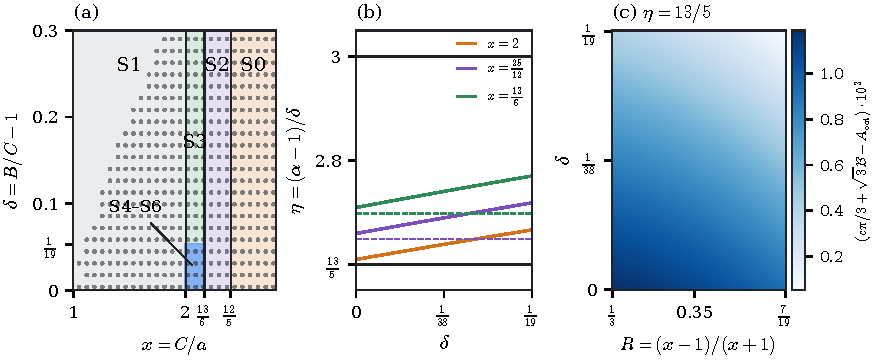
\includegraphics[width=\textwidth]{figures/fig-smaller-short.pdf}
 \caption{Parameter bounds from the gates. (a) The plane of the ratio $x=C/a$ and the displacement
 $\delta=B/C-1$. The dots are computed points of the equal-secant locus
 \eqref{eq:ss-equal-secants} with $1\le\alpha<x$. Gate S1 removes $x\le2$, S0 removes $x\ge12/5$,
 S2 removes $13/6\le x<12/5$ and S3 removes $\delta\ge1/19$, leaving the box where S4 to S6 work.
 (b) On that box, the slope $\eta=(\alpha-1)/\delta$ of the locus for $x=2,25/12,13/6$ (solid),
 between the lower order $1+4x(x+1)/(7x+1)$ (dashed) and the upper order $3$ of
 \cref{lem:ss-orders}. (c) The score gap
 $c\pi/3+\sqrt3\,\mathfrak B(u_*;R,T,\delta)-\Aoct$ of gate S6 at $\eta=13/5$:
 it is positive throughout the box.}\label{fig:smaller-short}
\end{figure}

\begin{proposition}[Gate S0]\label{prop:ss-S0}
Every smaller-short window has $x<12/5$, $D>0$ and $E_L>0$.
\end{proposition}

\begin{proof}[Proof sketch]
Suppose $x\ge12/5$. The root gives $R_\tau=0$ and $w\ge3/4$, so the floor-weighted residual
$G=R_\tau+\frac12(w-\frac34)$ is nonnegative at the actual window. Large ratios force an asymmetric
outer bridge: the equal secants and $x\ge12/5$ give $\alpha/\beta<3/4$ and then
$D<\alpha(\alpha+\beta)$. The weighted envelope \eqref{eq:ss-envelope} applies (its factor stays
positive for $x>5/3$), so $G^*_\tau\ge0$ at the actual scale, and the two shape facts make
$G^*_\tau$ increase with $u$. At fixed $p$ its value at the zero scale is negative, and an endpoint argument
for the quadratic in $q$ gives a nonnegative value at $q_{\max}$; the move along $\tau=2$ keeps it
nonnegative. On the face reached, $u$ is raised to the ceiling $\hat u(x,\beta)$ (central face) or
$\bar u(x,\beta)$ (outer face), and the duration is reduced to the three tests $F(2,\cdot)$,
$F(8\tau_{\max}/9,\cdot)$, $F(\tau_{\max},\cdot)$ of \cref{sec:ss-machinery}. The three face
signs of \cref{prop:ss-face-S0} say that each test is negative on the region cut out by the
orders. This
contradiction gives $x<12/5$. For $x\le12/5$ the identities
\begin{align*}
  D-\bigl[(1+2x)\alpha^2-2x^2\alpha+1+2x\bigr]&=2(\beta-\alpha x)(\alpha-x),\\
  (1+2x)\alpha^2-2x^2\alpha+1+2x-D_0&=(\alpha-1)\bigl[(1+2x)(\alpha+1)-2x^2\bigr],
\end{align*}
with $D_0=2+4x-2x^2\ge2/25$, give $D\ge\alpha D_0>0$. Finally
$E_L=\lambda(2\rho Du-E)>0$, because $E$ is at most its envelope value
$(1+x)(u-1)+\frac1{1+x}+\rho(2x+1)$, which is less than $2\rho Du$.
\end{proof}

\begin{proposition}[Gate S1]\label{prop:ss-S1}
Every smaller-short window has $x>2$.
\end{proposition}

\begin{proof}[Proof sketch]
Suppose $1<x\le2$. In this range we combine the residual with the upper bound $\Gamma<9193/50000$. Moving the opposite turn changes the Casimir $\Gamma(t,v)$ computed at
the central reverse run, but the combination $\Gamma-\frac{7}{96}R_\tau$ does not increase along
the two moves of \eqref{eq:ss-envelope}: in $v$ it is concave with a nonpositive slope at the
actual point, and along $v=\mathcal U(s)$ its derivative is the derivative of $R_\tau$, which is
negative, times a factor that stays below zero. Since $R_\tau=0$ at the actual window,
\[
  \Gamma\ge\Gamma_*-\tfrac{7}{96}R^*_\tau
\]
at the actual scale, where $\Gamma_*$ is the Gram expression at
$(t_0,\mathcal U(t_0))$. At fixed $p$ the right side decreases in $q$, and along $\tau=2$ the slope
of $R^*_2$ in $q$ exceeds one, so the right side does not increase when the point moves to a face.
On the central face $q=q_c\le1/7$ and on the outer face $q=1/7\le q_c$, the face signs
$\Gamma_*-\frac{7}{96}R^*_\tau>9193/50000$ for every admissible duration
(\cref{prop:ss-face-S1}) contradict $\Gamma<9193/50000$.
\end{proof}

\begin{proposition}[Gate S2]\label{prop:ss-S2}
A smaller-short window with $x<12/5$ has $x<13/6$.
\end{proposition}

\begin{proof}[Proof sketch]
Suppose $13/6\le x<12/5$. The weight is now variable, $m=2-7\tau/(4\tau_{\max})\in[1/4,2)$, and
the weighted residual $G_\tau=R_\tau+m(w-3/4)$ is still nonnegative at the root. The envelope
applies with this weight, the scale polynomial is convex in $q$ with a negative value at the zero
scale, and the $\tau=2$ continuation reaches the face $q^*=\min\{q_c,1/7\}$. After raising $u$ to
the ceiling $u_C(x,\beta)$ on the central face, and to $u_s(x,\beta)$ or $\bar V(x)$ on the outer
face, the face signs $G_\tau<0$ of \cref{prop:ss-face-S2} give the contradiction.
\end{proof}

\begin{proposition}[Gate S3]\label{prop:ss-S3}
A smaller-short window with $2\le x\le13/6$ has $\delta<1/19$.
\end{proposition}

\begin{proof}[Proof sketch]
Suppose $\delta\ge1/19$. The displacement is penalized by the weight
$m=4(4-3\tau/\tau_{\max})/(5\alpha-1)$, with which $G_\tau=R_\tau+m(w-3/4)\ge0$ at the root. On
this range $\beta<2\alpha$, so $D=\alpha^2+1+2x+2\beta(\alpha-x)>5\alpha^2-4\alpha x+1+2x\ge
6-2x>0$. The same three moves reach the face $q^*=\min\{q_c,1/7\}$. The duration is reduced to two
tests, $F_0$ at $\tau=2$ and $F_1$ at $\tau=\tau_{\max}$, the norm is raised to a ceiling, and on
the central face a monotonicity in $\beta$ moves the point to the curve
$\beta=x+\frac{25x}{15x+36}(\alpha-1)$. The face signs $F_0,F_1<0$ of
\cref{prop:ss-face-S3} give the contradiction.
\end{proof}

\subsubsection{Gate S4: the small box and a floor for the Casimir}\label{sec:ss-S4}

After gates S0 to S3 the shape lies in $2<x<13/6$, $0\le\delta<1/19$. Gate S6 needs a two-sided
control of $\alpha$ in terms of $\delta$, and also a lower bound for $\kappa$, because the
completion term in \eqref{eq:ss-defect} is weighted by $\kappa+3/2$.

\begin{proposition}[Gate S4]\label{prop:ss-S4}
A smaller-short window with $2\le x\le13/6$ and $\delta\le1/19$ has $\alpha\le1+3\delta$ and
$\Gamma>1829/10000$.
\end{proposition}

\begin{proof}[Proof sketch]
The first inequality is \cref{lem:ss-orders}(c), proved by the integral comparison in
\cref{app:ss-orders}. For the second, the monotonicity used in gate S1, now with the constant $1/7$,
gives $\Gamma\ge\Gamma_*-R^*_\tau/7$ at the actual scale. The scale
is moved at fixed $p$, and along $\tau=2$, up to the central scale $q_c$, and the duration maximum
\eqref{eq:ss-duration} leaves the two functions
\[
  \Phi=\Gamma_*(q_c)-\tfrac17R^*_2(q_c),\qquad
  \Psi=\Phi-\tfrac17(\tau_{\max}-2)\bigl(w_*(q_c)-\tfrac34\bigr).
\]
Both decrease in $u$, so the norm may be raised to its ceiling $\bar u(x,\beta)$
(\cref{app:ss-secant}). The face sign $\min\{\Phi,\Psi\}>1829/10000$ on the closed box
$2\le x\le13/6$, $0\le\delta\le1/19$, $\frac{13}{5}\delta\le\alpha-1\le3\delta$
(\cref{prop:ss-face-S4}) concludes.
\end{proof}

With \cref{lem:ss-orders} the window now lies in the \emph{small-shape domain}
\begin{equation}\label{eq:ss-small}
  2\le x\le\tfrac{13}{6},\qquad 0\le\delta\le\tfrac1{19},\qquad
  1+\tfrac{13}{5}\delta\le\alpha\le1+3\delta,
\end{equation}
that is $\alpha=1+\eta\delta$ with $13/5\le\eta\le3$ when $\delta>0$, and $\alpha=1$ when
$\delta=0$. No division by $\delta$ is used, so the symmetric boundary $\delta=0$ is included.

\subsubsection{Gate S5: the root forces a negative shear}\label{sec:ss-S5}

The defect inequality compares the cost of the bridge with the angle it turns, and both are
governed by one number. Let $M$ be the relative frame of the bridge, from the central switch to
the far switch. After a fixed rotation that depends only on $x$, its lower row does not depend on
$\rho$, and $\det M=1$ then determines the upper row up to one real parameter $h$, the
\emph{shear}. Put $R_x=(x-1)/(x+1)$, $T_s=(\beta-\alpha)/(\beta+\alpha)$,
$\mathcal U_1=\mathcal U(r)=(3+R_x^2)/4$, $\mathcal U_2=\mathcal U(r_A)=(3+T_s^2)/4$ and the
anisotropy $\nu=\mathcal U_1/\mathcal U_2-1\ge0$. Then
\begin{equation}\label{eq:ss-shear}
  \sqrt3\,h=\frac{(\beta x-\alpha)\bigl((x+2)\alpha+(2x+1)\beta\bigr)}
  {(1+x)^2(\alpha^2+\alpha\beta+\beta^2)}
  -2\,\mathcal U_1\,(2\beta x-x-\alpha\beta)\,\frac{\rho}{1-\rho}
.
\end{equation}
This is a strictly decreasing function of the central scale $\rho$, and the
bridge cost \eqref{eq:ss-cost} is affine in it:
\begin{equation}\label{eq:ss-cost-shear}
  \cost_{\mathrm{br}}=H_0-J_0h,\qquad J_0=\frac{3u}{2\,\mathcal U_1},\qquad
  H_0=\frac{\sqrt3}{2}\Bigl[\Bigl(1+\frac{u}{\mathcal U_1}\Bigr)R_x
   +\Bigl(1+\frac{u}{\mathcal U_2}\Bigr)T_s\Bigr].
\end{equation}
Decreasing the shear increases the bridge cost. Gate S5 shows that the actual outer root is
compatible only with a negative shear.

\begin{proposition}[Gate S5]\label{prop:ss-S5}
A smaller-short window in the small-shape domain \eqref{eq:ss-small} has
$q>\frac{15}{16}q_c$, $\sqrt3hR_x+\frac72\nu<0$, $h<0$ and $-hR_x>2\nu$.
\end{proposition}

\begin{proof}[Proof sketch]
Suppose $q\le q_b:=\frac{15}{16}q_c$. With weight zero, \eqref{eq:ss-envelope} and
\eqref{eq:ss-scale} give $\mathcal R(u;p,q):=\mathcal C(p)+q\mathcal L(p)\ge0$ at $p=\tau q$,
where $2q\le p\le r_A$. The residual is affine and increasing in $u$
(\cref{app:ss-S5}). The integral ceiling gives $u<19/25$ on the small-shape domain, so
$\mathcal R(19/25;p,q)\ge0$. At fixed $q$, however, the residual is concave in $p/r_A$ on its
allowed interval. Its tangent at $p=r_A$ has two endpoint values, both negative by the
shape comparisons in \cref{app:ss-S5}. This is a contradiction, so $q>q_b$.
The ratio comparison in \cref{app:ss-shear} then gives $-\sqrt3hR_x>7\nu/2$.
Since $R_x>0$ and $\nu\ge0$, this implies $h<0$ and $-hR_x>2\nu$, using $7>4\sqrt3$.
\end{proof}

\subsubsection{Gate S6: the completion cost bound}\label{sec:ss-S6}

\begin{proposition}[Gate S6]\label{prop:ss-S6}
For a smaller-short window in the small-shape domain with $\Gamma>1829/10000$, $h<0$ and
$-hR_x>2\nu$,
\[
  \cost_{\mathrm{br}}+\Bigl(\kappa+\frac32\Bigr)\Bigl(\frac\pi3-\theta_{\mathrm{br}}\Bigr)>\Aoct .
\]
\end{proposition}

The proof lowers the left side in four steps to an explicit function of the shape.

\runin{Step 1: lowering $\kappa$.} Since $12\cdot\frac{1829}{10000}-(\frac{40}{27})^2
=\frac{23}{1822500}>0$, the floor of gate S4 gives $\kappa>\kappa_0=40/27$. Since
$\theta_{\mathrm{br}}<\pi/3$, we may replace $\kappa+3/2$ by $c=\kappa_0+3/2=161/54$.

\runin{Step 2: the angle in terms of the shear.} Let $\psi=\arctan(R_x/\sqrt3)+\arctan(T_s/\sqrt3)$
be the angle of the fixed lower row of the rotated frame, let $K=\nu+2+2\kappa_0/J_0$, and
\[
  \delta(h)=2\arctan\frac{\sqrt{h^2+\nu^2}-h}{K+\sqrt{K^2-\nu^2}}.
\]
In the rotated basis, $\mathcal A+i\sqrt3\mathcal B$ is, up to a positive factor and the rotation
by $\psi$, a quadratic polynomial in one unknown entry of the costate at the central switch. The
condition that its values stay on one side of the line through the origin at angle $\psi+\delta$
is a discriminant inequality, which holds at $\delta=\delta(h)$. This gives
$\theta_{\mathrm{br}}\le\psi+\delta(h)$ for the actual shear. With
\eqref{eq:ss-cost-shear}, the left side of the proposition is at least
$H_0+c(\pi/3-\psi)+\tilde F(\delta(h))$, where $\tilde F(\delta)=-J_0\tilde h(\delta)-c\delta$ and
$\tilde h$ is the inverse of $h\mapsto\delta(h)$.

\runin{Step 3: continuation to the central scale.} The shear decreases in $\rho$, and $\rho<r^2$.
Let $h_c<h<0$ be the shear at the central scale $\rho=r^2$ and $\omega_c=\delta(h_c)$.
Throughout $[\delta(h),\omega_c]$, the quantity $H=-\tilde h$ satisfies
$\nu<HR_x/2$ and $H\le-h_c<R_x^2$. Together with the norm ceiling
$u\le3/4+R_x^2/12$, these bounds make $\tilde F$ strictly decreasing, by the
loss comparison in \cref{app:ss-S6}. The left side is therefore at least the central score
\[
  \mathcal F_c=\cost_c+c\Bigl(\frac\pi3-\psi-\omega_c\Bigr),\qquad
  \cost_c=\sqrt3\Bigl[\frac{u(2\beta x-x-\alpha\beta)}{x(x+2)}+\frac{R_x+T_s}{2}\Bigr] .
\]
Here $\cost_c$ is the bridge cost \eqref{eq:ss-cost} at the
central scale.

\runin{Step 4: minimizing the shape bound.} The integral estimate for the additional angle in
\cref{app:ss-S6} and a norm floor $u_*(R_x,\delta)$ obtained from the mean and variance of a
reciprocal integral give
\[
  \mathcal F_c>\frac{c\pi}{3}+\sqrt3\,\mathfrak B(u_*;R_x,T_s,\delta),
\]
with $\mathfrak B$ the function of \cref{app:ss-S6}, retaining the exact fixed-row angles. It is
concave in $T_s$, and $T_s$ is monotone in $\eta$, so its minimum over $13/5\le\eta\le3$ is
attained at an endpoint. The bound decreases with displacement, and at the largest displacement
it is concave in $R_x$. Its minimum is therefore at one of four corners
(\cref{prop:ss-face-S6}, \cref{fig:smaller-short}(c)), where a reciprocal-integral bound gives
$\mathfrak B>9/4000$. The direct octagon comparison of
\cref{lem:octagon-cost-comparison}, with $c/3=161/162$, now gives
\[
 \Aoct<\frac{c\pi}{3}+\frac{9\sqrt3}{4000}<\mathcal F_c.
\]


\subsubsection{Proof of \texorpdfstring{\cref{thm:m2-smaller-short}}{the theorem}}\label{sec:ss-assembly}

Let a smaller-short window be given. Gate S0 gives $x<12/5$, gate S1 gives $x>2$, and gate S2
then gives $x<13/6$. Gate S3 gives $\delta<1/19$, gate S4 gives $\alpha\le1+3\delta$ and
$\Gamma>1829/10000$, and \cref{lem:ss-orders} gives $\alpha\ge1+\frac{13}{5}\delta$. So the
window lies in the small-shape domain \eqref{eq:ss-small}. Gate S5 gives $h<0$ and
$-hR_x>2\nu$, and gate S6 then contradicts the window defect \eqref{eq:ss-defect}. \qed

\subsection{Estimates for the smaller-short window}\label{app:short-estimates}

This subsection gives the scalar inequalities behind \cref{sec:smaller-short}, organized by the
gate that uses them. They are identities between rational functions, and inequalities proved by
exhibiting a difference as a sum of terms of known sign, by the sign of a derivative on an
interval, or by monotonicity or convexity in one variable at a time. The face signs for gates
S0 to S4 in \cref{app:ss-faces} reduce, one variable at a time, to polynomials in one or two
variables, mostly of degree at most eight. We give the reductions and final signs; every
polynomial is specified by the rational expressions at the face where it is evaluated.
Gates S5 and S6 use the direct concavity and derivative comparisons given below.
Throughout, $\operatorname{Sec}$, $g_B$ and $\mathcal U$ are as in \cref{sec:ss-window}, and the
variables are those of \cref{tab:ss-variables}.

\subsubsection{Secants and the incoming norm}\label{app:ss-secant}

By \eqref{eq:ss-secant}, $(P_0-A_0)\operatorname{Sec}(A_0,B_0,P_0)$ is the integral of $g_{B_0}$
over $[A_0,P_0]$, hence additive over adjacent intervals, and by \eqref{eq:ss-g} every secant lies
in $[3/4,1]$. The function $g_{B_0}$ decreases on $(0,B_0]$ and increases on $[B_0,\infty)$. For
the bridge norm, \eqref{eq:ss-g} gives
\begin{equation}\label{eq:ss-u-integral}
  u-\frac34=\frac{1}{4(\beta-1)}\int_1^\beta\frac{(s-x)^2}{(s+x)^2}\,\dd s .
\end{equation}

\runin{The central value.} Normalize the integration variable by $x$ and put $a=1/x$.
Then
\[
 V(x)=\frac{1}{1-a}\int_a^1g(s)\,\dd s,\qquad g(s)=1-\frac{s}{(1+s)^2}.
\]
Since $g$ strictly decreases on $(0,1)$, adding $[0,a]$ strictly raises the average. Hence
$V$ increases with $x$ and
\[
 V(x)<V_\infty:=\int_0^1g(s)\,\dd s=\frac32-\log2,
 \qquad \lim_{x\to\infty}V(x)=V_\infty.
\]
With $z=(x-1)/(x+1)$ one also has $2x/(1+x)=1+z$ and
\[
  V(x)-\frac34=\operatorname{Sec}(1,x,x)-\frac34=\frac12+\frac z4-\frac{(1+z)\log(1+z)}{2z}.
\]
A lower bound for $\log(1+z)$ is therefore an upper bound for $V$.
The weighted Jensen bound $L_J(z)$ of \cref{lem:m2-logs}(c) gives
\[
 V(x)-\frac34<U(z):=\frac12+\frac z4-\frac{(1+z)L_J(z)}{2z}.
\]
This proves the ceiling used below,
\[
 V_G(x)=\frac34+\frac{(x-1)^2(71x^2+48x+1)}{96x(x+1)(13x^2+14x+3)},
\]
because direct subtraction gives the positive difference
\[
 V_G(x)-\frac34-U(z)=
 \frac{(x-1)^6}{96x(3x+1)(13x^2+14x+3)(21x^2+18x+1)}>0.
\]
Finally
\[
 \bar V(x)-V_G(x)=\frac{(x-1)^3(11x^2+96x+13)}{96x(x+1)(35x+13)(13x^2+14x+3)}\ge0
\]
gives $V\le\bar V=\frac34+\frac{2(x-1)^2}{(x+1)(35x+13)}$.

\runin{Ceilings and floors.} Splitting \eqref{eq:ss-u-integral} at $x$, bounding the integral over
$[1,x]$ by $(x-1)(\bar V-\frac34)$ or by a sharper rational bound, and bounding $(s-x)^2/(s+x)^2$
on $[x,\beta]$ by a quadratic or linear function of $s-x$, gives the rational ceilings of the
bridge norm used by the gates:
\begin{align*}
  \bar u&=\tfrac34+\tfrac{1}{\beta-1}\Bigl[\tfrac{2(x-1)^3}{(x+1)(35x+13)}
   +\tfrac{(\beta-x)^3}{48x^2}\Bigr],&
  \hat u&=\tfrac34+\tfrac{(x-1)^2(\beta+7x-8)}{4(x+1)(35x+13)(\beta-1)},\\
  u_\ell&=\tfrac34+\tfrac{(x-1)^2(\beta+15x-16)}{8(x+1)(35x+13)(\beta-1)},&
  u_C&=\tfrac34+\tfrac{680(x-1)^3+3(x+1)^2(\beta-x)}{9600(x+1)^2(\beta-1)},\\
  u_s&=\tfrac34+\tfrac{1}{\beta-1}\Bigl[\tfrac{17(x-1)^3}{240(x+1)^2}+\tfrac{\beta-x}{1200}\Bigr],&
  u_O&=\tfrac34+\tfrac{(x-1)^2(x+\beta-2)}{(\beta-1)(x+1)(35x+13)},\\
  u_{CB}&=\tfrac34+\tfrac{(x-1)(V_G(x)-3/4)+(\beta-x)/5808}{\beta-1},
\end{align*}
together with the floor $u_f=\frac34+\frac{(x-1)^2}{28(x+1)^2}$ and the integral floor $u_*$ of
gate S6 (\cref{app:ss-S6}). The ceiling $\bar u$ holds for all $1<x\le\beta$; each of the others
holds on the shapes where its gate uses it.

\subsubsection{Orders and the comparison argument}\label{app:ss-orders}

Normalize the shape by $\beta$: put $\ell=1/x$, $p_1=\alpha/\beta$, $q_1=x/\beta$ and
$\operatorname{avg}(p,q)=\operatorname{Sec}(p,1,q)$, the mean of $g(s)=1-s/(1+s)^2$ over $[p,q]$, with $\operatorname{avg}(p,p)=g(p)$ by continuity.
The equal secants \eqref{eq:ss-equal-secants} read
$\operatorname{avg}(\ell,1/q_1)=\operatorname{avg}(p_1,q_1)$. An order compares $p_1$ with a
\emph{barrier} $P(z)$, a differentiable function with $P(1)=\ell$, through the comparison function
\[
  \Phi(z)=\operatorname{avg}\bigl(P(z),z\bigr)-\operatorname{avg}(\ell,1/z),\qquad\Phi(1)=0 .
\]
Because $\operatorname{avg}$ decreases in its left end, the sign of $\Phi(q_1)$ decides whether
$p_1$ lies above or below $P(q_1)$.

\begin{lemma}[First contact]\label{lem:ss-first-contact}
Let $a<1$ and let $\Phi$ be continuous on $[a,1]$ with $\Phi(1)=0$. If $\Phi$ has a negative
derivative at each of its zeros in $(a,1]$, then $\Phi>0$ on $(a,1)$.
\end{lemma}

\begin{proof}
Since $\Phi(1)=0$ and $\Phi'(1)<0$, $\Phi>0$ on some interval $(1-\varepsilon,1)$. If
$\Phi(z_0)\le0$ for some $z_0\in(a,1)$, then $\Phi$ has a zero in $[z_0,1-\varepsilon]$; let $z^*$
be the largest one. Then $\Phi>0$ on $(z^*,1)$ and $\Phi(z^*)=0$, so $\Phi'(z^*)\ge0$, a
contradiction.
\end{proof}

At a zero of $\Phi$ both averages equal a common value $u$, and differentiation gives
\begin{multline*}
  \Phi'(z)\,(z-P(z))\,z\,(x-z)\\
  =-P'(z)\bigl(g(P(z))-u\bigr)z(x-z)-\bigl(u-g(z)\bigr)\bigl((2z-P(z))x-z^2\bigr).
\end{multline*}
Thus the sign at a contact depends on the ratio of the two endpoint gaps. We first bound this
ratio by comparing positive weights in its integral representation.

\begin{lemma}[Endpoint gaps]\label{lem:ss-endpoint-gaps}
For $0<p<q\le1$, put $m=\operatorname{avg}(p,q)$. Then
\[
 \frac{3-2p-q}{3-p-2q}
 +\frac{q-p}{6}<\frac{g(p)-m}{m-g(q)}
 <\frac{\log2-1/2}{3/4-\log2}.
\]
\end{lemma}

\begin{proof}
Write $d=q-p$ and
\[
 h(t)=-g'(p+dt)=\frac{1-p-dt}{(1+p+dt)^3},\qquad 0<t<1.
\]
Integration by parts gives
$g(p)-m=d\int_0^1(1-t)h(t)\,\dd t$ and
$m-g(q)=d\int_0^1th(t)\,\dd t$.
Their ratio is $(1-\mu)/\mu$, where $\mu$ is the mean of $t$ with weight $h$.
Multiplying a positive weight by a decreasing function lowers this mean: its covariance
with $t$ is the integral of $(t-s)(a(t)-a(s))/2$ against two copies of the probability measure,
and is nonpositive. Apply this to the linear weight $1-p-dt$ and the strictly decreasing
factor $(1+p+dt)^{-3}$. The ratio for the linear weight is
$(3(1-p)-d)/(3(1-p)-2d)$, giving the first term of the lower bound.

More generally, put $b=1-p$. The quotient $h(t)/[(b-dt)(1-\eta t)]$ decreases whenever
$0\le\eta\le3d/(1+p+4d)$: its logarithmic derivative has the sign of
$\eta(1+p+4dt)-3d$, which is negative for $0<t<1$. The same covariance comparison gives
\begin{equation}\label{eq:ss-gap-tilt}
 \frac{g(p)-m}{m-g(q)}>
 \mathcal Q_\eta(p,q):=
 \frac{\int_0^1(1-t)(b-dt)(1-\eta t)\,\dd t}
      {\int_0^1t(b-dt)(1-\eta t)\,\dd t}.
\end{equation}
These weights are positive on the interior, since $\eta<3/4$.
For the quantitative improvement take $\eta=d/2$, which is admissible because
$1+p+4d<6$. If $\mu_0$, $m_2$ and $\sigma^2$ are the mean, second moment and variance
for the linear weight, direct integration gives
\[
 \frac{\sigma^2}{\mu_0^2}
 =\frac13+\frac{d(6b-5d)}{6(3b-2d)^2}>\frac13,
\]
because $0<d\le b$. Tilting increases the gap ratio by
\[
 \frac{\eta\sigma^2}{\mu_0(\mu_0-\eta m_2)}
 >\frac{\eta\sigma^2}{\mu_0^2}>\frac\eta3=\frac d6.
\]
The denominator is positive, as it is a positive multiple of the first moment of the tilted
weight. This proves the stated refinement.

For the upper bound compare $h$ with $h_0(t)=(1-t)/(1+t)^3$. The quotient
\[
 \frac{h(t)}{h_0(t)}
 =\frac{1-p-dt}{1-t}\left(\frac{1+t}{1+p+dt}\right)^3
\]
increases: the two factors have derivatives with numerators $1-q\ge0$ and
$1+2p-q>0$, respectively. Thus $h$ has a larger mean than $h_0$ and a smaller gap ratio.
The latter ratio is exactly $(\log2-1/2)/(3/4-\log2)$. Its numerator and denominator are
positive integrals of $(1-t)h_0(t)$ and $th_0(t)$, respectively, so no numerical logarithm
bound is needed.
\end{proof}

\runin{The global upper order.} Take $k=5/4$ and $P(z)=\ell+k(1-z)$. If $P(q_1)\ge q_1$, the
upper bound $p_1\le P(q_1)$ is automatic from $p_1<q_1$. On the interval $P(z)<z$, put
\[
 a=1-\ell,\qquad \theta=\frac{1-z}{a},\qquad
 R_0=\frac{3-2P(z)-z}{3-P(z)-2z}.
\]
Here $0<a<1$ and $0\le\theta<4/9$, since $P(z)<z$.
The following identity makes the contact sign positive:
\begin{align*}
 &kR_0z(x-z)-\bigl((2z-P(z))x-z^2\bigr)\\
 &\quad=\frac{a}{4(1-a)(4+3\theta)}\Bigl[
 1+6\theta^2+7(3\theta-1)^2\\
 &\qquad\qquad
 +6(1-a)\theta\bigl(2(4-9\theta)+7\theta^2\bigr)
 +6(1-a)^2\theta^2(4-7\theta)\Bigr]>0.
\end{align*}
Every factor in the bracket is nonnegative, and the constant term is positive.
By the lower gap bound of \cref{lem:ss-endpoint-gaps}, $\Phi'>0$ at every zero,
including $z=1$. Apply \cref{lem:ss-first-contact} to $-\Phi$: then $\Phi<0$ to the left of
one, and decreasing the left endpoint of the average gives $p_1<P(q_1)$ if $q_1<1$.
This proves the upper order $\alpha\le\beta/x+\frac54(\beta-x)$ of \cref{lem:ss-orders}(b).
If $q_1=1$, equality of the two averages forces $p_1=\ell$, so the same bound holds.

\runin{The upper order for $x\le5$.} Now take $k=9/8$ and $P(z)=\ell+k(1-z)$.
Again only the interval $P(z)<z\le1$ needs a comparison. Put
\[
 a=1-\ell,\qquad 0\le\theta=\frac{1-z}{a}<\frac8{17},\qquad
 E=1+\frac78\theta,\qquad D=1-\frac{17}{8}\theta>0.
\]
Let $R_0=(3-2P(z)-z)/(3-P(z)-2z)$ and define the normalized contact expression
\[
 \mathcal N(\ell,\theta)=\frac{E(1-a)}a
 \left[kR_0z(x-z)-\bigl((2z-P(z))x-z^2\bigr)\right].
\]
This expression does not decrease in $\ell$. Indeed,
\[
 \partial_\ell\mathcal N
 =\frac\theta{32}\left[73\theta^2-186\theta+80
                   +2\ell\theta(40-73\theta)\right]\ge0.
\]
On $0\le\theta<1/2$, the first quadratic decreases and is at least its value $21/4$ at
$1/2$; also $40-73\theta>7/2$.
By the refined gap bound, the actual normalized contact sign is strictly greater than
\[
 \mathcal N+\frac3{16}aDE(1-a\theta)(1+\ell\theta)
 \ge\mathcal N+\frac3{16}aD(1-\theta).
\]
For $1<x\le3$, use $\ell\ge1/3$ and the identity
\[
 \mathcal N(1/3,\theta)
 =\frac94\left(\theta-\frac13\right)^2
       +\frac{\theta(30+53\theta+292\theta^2)}{576}>0.
\]
For $3\le x\le5$, use $a\ge2/3$ and $\ell\ge1/5$. The lower bound is then at least
\begin{align*}
 \mathcal N(1/5,\theta)+\frac18D(1-\theta)
 &=\frac{27}{8}\left(\theta-\frac13\right)^2
    +\theta\left(\frac5{64}-\frac{13\theta}{160}\right)
    +\frac{73\theta^3}{200}\\
 &\ge\frac{27}{8}\left(\theta-\frac13\right)^2+\frac{3\theta}{80}>0,
\end{align*}
since $\theta<1/2$. The contact derivative is therefore positive in both ranges.
The same first-contact argument as for $k=5/4$ gives
$\alpha\le\beta/x+\frac98(\beta-x)$, including equality when $\beta=x$.

\runin{The upper order in the small box.} We prove \cref{lem:ss-orders}(c).
Here $q_1=1/(1+\delta)\ge19/20$, so it suffices to compare barriers on $19/20\le z\le1$.
If $x\le16/9$, the upper order just proved gives
$\alpha\le1+(1+9x/8)\delta\le1+3\delta$.

For $16/9\le x\le2$, take $P(z)=\ell+1-z$, put $a=1-\ell$ and $\theta=(1-z)/a$,
and use \eqref{eq:ss-gap-tilt} with $\eta=(z-P(z))/2$.
We have $a\ge7/16$ and $\theta\le4/35<1/8$. Direct integration of the tilted linear weight gives
\begin{align*}
 &\mathcal Q_\eta(P(z),z)z(x-z)-\bigl((2z-P(z))x-z^2\bigr)\\
 &\quad=\frac{a^2(1-2\theta)}{(1-a)(4a\theta^2+4\theta-a+4)}
 \bigl[1-6\theta-6\theta^2-2a(1-a)\theta^3\bigr]>0.
\end{align*}
The bracket exceeds $1-6/8-6/64-1/1024>0$, using $a(1-a)\le1/4$.
First contact therefore gives $\alpha\le\beta/x+(\beta-x)=1+(1+x)\delta\le1+3\delta$.

It remains to consider $2\le x\le13/6$, so $6/13\le\ell\le1/2$.
Take $P(z)=\ell(3-2z)$ and, at a contact, put
$p=P(z)$, $s=1-z$, $b=1-p$ and $d=z-p=b-s$.
The maximal tilt $\eta=3d/(1+p+4d)$ in \eqref{eq:ss-gap-tilt} has the ratio
\[
 \mathcal T(b,s):=\mathcal Q_\eta(p,z)=\frac ND,\qquad
 \begin{aligned}
 N&=9b^2-10bs-5s^2+8b+4s,\\
 D&=3b^2-2bs-7s^2+4b+8s.
 \end{aligned}
\]
We compare $2\ell\mathcal T$ with
$M=1+(z-p)/[z(1-\ell z)]$, since their difference has the sign of the contact derivative.
On this rectangle $9/20\le b\le7/13$, $0\le s\le1/20$ and $p\le11/20$.
Also $d/b\ge8/9$, so the linear-weight ratio is at least $19/11$ and
$\mathcal T>17/10$. The positive expressions above give
\[
 D>\frac{12}{5},\qquad N_b<18,\qquad D_b>\frac{13}{2},\qquad
 \mathcal T_b=\frac{N_b-\mathcal T D_b}{D}<3.
\]
For the first inequality use $D\ge b(3b+4)$; for the last use
$18-(17/10)(13/2)<3(12/5)$. Consequently
\[
 \partial_p(p\mathcal T)=\mathcal T-p\mathcal T_b>\frac1{20},\qquad
 M_\ell=\frac{(z-1)(z+3)}{z(1-\ell z)^2}\le0.
\]
Thus $2\ell\mathcal T-M$ increases in $\ell$, and it suffices to take $\ell=6/13$.

Along this edge $b=(7-12s)/13$. Write $k=12/13$ for $b_z$.
The two quadratics satisfy
$N_{zz}=18k^2+20k-10>0$ and $D_{zz}=6k^2+4k-14<0$.
Their endpoint values and the upper tangent to $D$ at $z=1$ give
\[
 N_z\ge N_z(19/20)>16,\qquad
 D_z\le D_z(19/20)<\frac18,\qquad D<\frac{31}{10}.
\]
Moreover $\mathcal T<5/2$, since
$5D-2N=b(4-3b)+s(10b+32-25s)>0$.
It follows that
\[
 \mathcal T_z=\frac{N_z-\mathcal T D_z}{D}
 >\frac{16-5/16}{31/10}>5.
\]
On the same edge,
\[
 M_z=\frac{6(25z^2-36z+39)}{z^2(13-6z)^2}<4:
\]
its numerator is at most $168$, while $z(13-6z)>13/2$.
Therefore $(2\ell\mathcal T-M)_z>8/13>0$, and the smallest value is at $z=19/20$.
At that corner $s=1/20$ and $d=23/52$. The inequality
$(23/52)^2>39/200$ gives $N-2D=3d^2-6s(2-s)>0$, so $\mathcal T>2$.
Also $d<4/9$ and $z(1-\ell z)>8/15$, giving $M<11/6<24/13=4\ell$.
The contact sign is positive. First contact gives $p_1\le\ell(3-2q_1)$, or
$\alpha\le3\beta/x-2=1+3\delta$, as required.

\runin{Feasibility of a lower barrier.} The lower-order proofs below use the following observation.
Suppose $0<z_m<1$, $P(1)=\ell$, $P(z_m)=z_m$ and $P(z)<z$ for $z_m<z\le1$.
If its comparison function $\Phi$ is positive on $(z_m,1)$, the actual equal-secant shape
must have $q_1>z_m$. Indeed, put
\[
 H(b)=\int_\ell^b g(s)\,\dd s-(b-\ell)g(b),\qquad b\ge1.
\]
This decreases because $H'(b)=-(b-\ell)g'(b)\le0$.
At the actual shape, $\operatorname{avg}(\ell,1/q_1)=\operatorname{avg}(p_1,q_1)>g(q_1)$,
so $H(1/q_1)>0$, using $g(1/q_1)=g(q_1)$.
It follows that $\operatorname{avg}(\ell,1/z)>g(z)$ for $q_1\le z\le1$.
If $q_1\le z_m$, this makes $\Phi(z_m)<0$, contrary to continuity and
$\Phi>0$ on $(z_m,1)$. Thus $q_1>z_m$.

\runin{The strong lower order.} We prove \cref{lem:ss-orders}(a), without a restriction on $x$.
Put $a=1-\ell\in(0,1)$ and $k=4(2-a)/(8-a)\in(0,1)$, and take $P(z)=\ell+k(1-z)$.
For $p=P(z)<z$, use the relative endpoint deficits
\[
 b=1-p,\qquad r=\frac{1-z}{1-p},\qquad
 b=\frac{a}{1+kr},\qquad 0<b<1,\quad 0\le r<1.
\]
Write $\mathcal R(b,r)$ for the endpoint-gap ratio on $[1-b,1-br]$.
At fixed $r$ its integral weight, up to a constant factor, is
\[
 w_b(t)=\frac{v(t)}{(2-bv(t))^3},\qquad v(t)=1-(1-r)t.
\]
The ratio $w_{b_2}/w_{b_1}$ decreases in $t$ when $b_2>b_1$: its logarithmic derivative
with respect to $v$ is $6(b_2-b_1)/[(2-b_1v)(2-b_2v)]>0$.
The covariance argument in \cref{lem:ss-endpoint-gaps} therefore shows that $\mathcal R$
increases in $b$.

Simpson's bound for the reciprocal integral gives a convenient upper estimate. In the form
\[
 L(y)=\frac{y-1}{6}\left(1+\frac8{1+y}+\frac1y\right),\qquad
 (L-\log)'(y)=\frac{(y-1)^4}{6y^2(1+y)^2},
\]
it follows directly that $\log y<L(y)$ for $y>1$.
Substitute $y=(1+q)/(1+p)$ in
\[
 \operatorname{avg}(p,q)=1+\frac1{(1+p)(1+q)}
                         -\frac{\log y}{q-p}.
\]
The resulting lower mean $m_L$ lies above $g(q)$: for $p=1-b$, $q=1-br$,
\[
 m_L-g(q)=\frac{b^2(1-r)\,[4+8r-br(5+r)]}
 {6(2-b)(2-br)^2(4-b-br)}>0,
\]
since the bracket is at least $4+3r-r^2>0$.
The gap ratio decreases as the mean increases, so
\[
 \mathcal R(b,r)<\widehat{\mathcal R}(b,r):=
 \frac{2-br}{2-b}\,
 \frac{8+4r-b(1+5r)}{4+8r-br(5+r)}.
\]

The slope satisfies
$k-(1-a/2)=a(2-a)/[2(8-a)]>0$.
Thus $b\le b_*:=a/[1+(1-a/2)r]$, and comparison of the weights followed by the last bound gives
$\mathcal R(b,r)<\widehat{\mathcal R}(b_*,r)$.
Set $B=1+(1-r)(2/k-1)/[1+(2-a)r]$ and write
\begin{align*}
 H_*&=4+(12-7a)r+(8-5a)r^2,\\
 Q&=(1+r)\{4(1-a)(7r+1)+a(9r+11)\}+2a(1-a)r(5-r).
\end{align*}
Multiplication of the two fractions gives the positive-product identity
\[
 B-\widehat{\mathcal R}(b_*,r)
 =\frac{ar(1-r)Q}{2(2-a)(1+r)(1+(2-a)r)H_*}\ge0.
\]
Here $H_*,Q>0$, so $\mathcal R<B$, also when $r=0$ by the strict Simpson bound.

It remains to compare this upper bound with the contact threshold
$M=1+(z-p)/[z(1-\ell z)]$.
Put $h=k-a$ and
\[
 B_0=1+\frac{(1-r)(2/k-1)}{1+(1+h)r}.
\]
Since $k<1$, we have $B\le B_0$, while substitution of
$p=1-a/(1+kr)$ and $z=1-ar/(1+kr)$ gives
\[
 M-kB_0=
 \frac{r\bigl[(1-r)(2-k(1+h))+r(1-k)(1+h)(2+h)\bigr]}
 {(1+hr)(1+(1+h)r)}\ge0.
\]
Here $-1<h<k<1$ and $2-k(1+h)>2-k(1+k)=(1-k)(k+2)>0$.
Consequently $k\mathcal R<kB\le kB_0\le M$, so $\Phi'<0$ at every zero, including $z=1$.
First contact gives $\Phi>0$ between the crossing $P(z_m)=z_m$ and $1$.
The preceding feasibility argument, applied to this crossing,
shows that the actual $q_1>z_m$.
Thus $p_1>P(q_1)$ when $q_1<1$; when $q_1=1$, $p_1=\ell$.
Multiplying by $\beta$ proves the claimed lower order.

\runin{The quadratic lower order.} For \cref{lem:ss-orders}(d), retain $a=1-\ell$ and
$k=4(1+\ell)/(7+\ell)$, but curve the barrier:
\[
 P(z)=\ell+ks+\frac{\ell s^2}{1+3s},\qquad s=1-z.
\]
Here $6/13\le\ell\le1/2$, so
\[
 \frac12\le a\le\frac7{13},\qquad
 \frac34<k\le\frac45,\qquad \frac15<k-a\le\frac3{10}.
\]
For $p=P(z)<z$, put
\[
 K=k+\frac{\ell s}{1+3s},\qquad
 j=-P'(z)=K+\frac{\ell s}{(1+3s)^2},\qquad
 r=\frac{s}{1-p}.
\]
Then $0\le r<1$, $b=1-p=a/(1+Kr)$ and $s=ar/(1+Kr)$.
The condition $p<z$ gives $s<a/(1+k)<1/3$, hence $k\le K<9/10$ and $j\ge k>3/4$.
At a contact it suffices to prove $j\mathcal R(b,r)<M(K)$, where
\[
 M(v)=1+\frac{(1-r)(1+vr)}{(1+(v-a)r)(1+(v+\ell)r)}.
\]
This is the contact threshold $1+(z-p)/[z(1-\ell z)]$ when $v=K$.

First keep the positive gain in the preceding comparison. With the same $B,B_0,H_*,Q$ as
there, put $E=B-\widehat{\mathcal R}(b_*,r)\ge0$.
Since $K\ge k$, comparison of the weights still gives
$\mathcal R(b,r)<B-E$.
Write $D=M(k)-kB_0$. The preceding positive-product identity and the bounds on $k-a$ give
\[
 D\ge\frac{r\bigl[\frac{19}{20}(1-r)+\frac12r\bigr]}
 {(1+3r/10)(1+13r/10)}.
\]
Indeed its two numerator factors $2-k(1+k-a)$ and
$(1-k)(1+k-a)(2+k-a)$ exceed $19/20$ and $1/2$.
The remaining two gains satisfy
\begin{equation}\label{eq:ss-quadratic-gains}
 k(B_0-B)\ge\frac{r(1-r)}{5(1+2r)^2},\qquad
 jE\ge\frac{r(1-r)}{5(1+2r)^2}.
\end{equation}
For the first, subtract the two fractions:
\[
 k(B_0-B)=\frac{r(1-r)(2-k)(1-k)}
 {(1+(1+k-a)r)(1+(2-a)r)}.
\]
Both denominator factors are at most $1+2r$ and $(2-k)(1-k)>1/5$.
For the second, the positive expressions for $Q,H_*$ give
\[
 Q\ge7(1+r)(1+3r/2),\qquad H_*\le4(1+2r)^2.
\]
Together with $a/[2(2-a)]\ge1/6$ and $2-a\le3/2$, these imply
$E\ge7r(1-r)/[24(1+2r)^2]$. Now use $j>3/4$ and $7/32>1/5$.

Next bound the two costs of curving the barrier. Set $\eta=K-k$. The identities for $s$ give
\[
 \eta=\frac{\ell ar}{1+(K+3a)r},\qquad
 j-k=\frac{\ell ar\,[2+(2K+3a)r]}{(1+(K+3a)r)^2}.
\]
Since $\ell a\le1/4$, $K+3a>9/4$ and $2K+3a<7/2$,
\begin{equation}\label{eq:ss-quadratic-costs}
 \eta\le\frac{r}{4(1+9r/4)},\qquad
 j-k\le\frac{r(2+7r/2)}{4(1+9r/4)^2}.
\end{equation}
Also $2/k-1<8/5$ and $2-a>7/5$, so $B\le(13-r)/(5+7r)$.
For the change in $M$, put
\[
 F(v)=\frac{1+vr}{(1+(v-a)r)(1+(v+\ell)r)},\qquad k\le v\le K.
\]
With $u=1+(v-a)r\ge1+r/5$, direct differentiation gives
\[
 0\le-F'(v)=\frac{r(u^2+2aru+ar^2)}{u^2(u+r)^2}\le\frac r u.
\]
For the last inequality compare the three numerator terms with those of $u(u+r)^2$,
using $u\ge1>a$. Integration over $[k,K]$, followed by \eqref{eq:ss-quadratic-costs}, yields
\[
 0\le M(k)-M(K)\le\frac{(1-r)\eta r}{1+r/5}
 \le\frac{r^2(1-r)}{4(1+9r/4)(1+r/5)}.
\]

For $r>0$, normalize by $S=(1+2r)^2/r$.
The three denominator comparisons
\begin{gather*}
 (1+3r/10)(1+13r/10)\le1+2r,\\
 1+2r\le1+9r/4,\\
 (1+9r/5)(1+r/5)\ge1+2r
\end{gather*}
give
\begin{align*}
 SD&\ge\left(\frac{19}{20}-\frac9{20}r\right)(1+2r),\\
 S(j-k)B&\le\frac{(4+7r)(13-r)}{8(5+7r)}
       \le\frac{13}{10}+\frac r{10}+\frac3{10}r(1-r),\\
 S\bigl(M(k)-M(K)\bigr)&\le\frac{r(1-r)(1+9r/5)}4.
\end{align*}
The second upper bound follows by division:
\[
 \frac{(4+7r)(13-r)}{8(5+7r)}
 =\frac{13}{10}+\frac{3r}{40}+\frac{7r(1-r)}{5(5+7r)}.
\]
Combining these estimates with \eqref{eq:ss-quadratic-gains} gives
\begin{align*}
 S\bigl(M(K)-j\mathcal R(b,r)\bigr)
 &>\left(\frac{19}{20}-\frac9{20}r\right)(1+2r)+\frac25(1-r)\\
 &\quad-\left(\frac{13}{10}+\frac r{10}+\frac3{10}r(1-r)\right)
       -\frac{r(1-r)(1+9r/5)}4\\
 &=\frac{1+r^3}{20}+\frac25r(1-r)^2>0.
\end{align*}
When $r=0$, $j=k$, $M(K)=2$ and $E=0$, while the Simpson bound still gives
$\mathcal R<B=2/k$. Thus the contact derivative is negative in this case as well.

The function $P(z)-z$ decreases strictly and has a unique zero $z_m\in(0,1)$.
First contact gives $\Phi>0$ on $(z_m,1)$; the same feasibility function $H$ as above excludes
$q_1\le z_m$. Hence $p_1>P(q_1)$ for $q_1<1$, with equality for $q_1=1$.
Finally, $s=\delta/(1+\delta)$ and multiplication by $\beta=x(1+\delta)$ transform the barrier into
\[
 \beta P(q_1)=1+(1+xk)\delta+\frac{\delta^2}{1+4\delta},
\]
which is the order claimed in part (d).

\subsubsection{The outer scale bound}\label{app:ss-scale}

\begin{lemma}[Reverse-centre scale bound]\label{lem:ss-outer-scale}
At a reverse centre with neighbour ratios $0<r,t<1/2$, scale $0<\rho<rt$, and norms
$3/4\le u\le\mathcal U(r)$, $3/4\le v\le\mathcal U(t)$ and the stationarity
$E=1+r+t-\rho+\log\frac{\rho}{rt}-\frac{1-u}{r}-\frac{1-v}{t}$, the inequality
$(4uv-E^2)/(16(1-\rho)^2)<9193/50000$ implies $\rho<1/7$.
\end{lemma}

\begin{proof}
Assume $\rho\ge1/7$. First consider the pairing $E_0$ at $u=v=3/4$.
With $\sigma=rt$ and $\chi=r+t$, the inequalities $r,t<1/2$ give
$\chi\le1/2+2\sigma$, so
\[
 E_0=1-\rho+\log\frac\rho\sigma+\chi\left(1-\frac1{4\sigma}\right)
 \ge L(\sigma):=1-\rho+\log\frac\rho\sigma+2\sigma-\frac1{8\sigma}.
\]
Since $L'(\sigma)=(4\sigma-1)^2/(8\sigma^2)\ge0$ and $\sigma>\rho$,
$E_0\ge L(\rho)=1+\rho-1/(8\rho)>0$. The pairing increases with either norm, hence $E\ge E_0>0$.

The switch ceilings also give $E<-1+2r+2t-rt\le3r/2$, and symmetrically $E\le3t/2$.
For the first inequality use that $\log\rho-\rho$ increases for $\rho<1$; for the second use
$-1+r/2+2t-rt=(1-2t)(r/2-1)\le0$. Consequently
\[
 \partial_u(4uv-E^2)=4v-\frac{2E}{r}\ge4v-3\ge0,
\]
and the analogous derivative in $v$ is nonnegative. Lowering both norms to $3/4$ therefore
lowers the Gram quotient. At those norms,
$\partial_rE_0=(r-1/2)^2/r^2\ge0$, and likewise for $t$.
Letting both ratios increase to $1/2$ raises the positive pairing and lowers the quotient again:
\[
 \frac{4uv-E^2}{16(1-\rho)^2}\ge
 G(\rho):=\frac{9/4-B(\rho)^2}{16(1-\rho)^2},\qquad
 B(\rho)=1-\rho+\log4\rho .
\]
On $[1/7,1/4)$ the function $B$ is positive, and $G$ increases by the fixed-$S$
monotonicity in the proof of \cref{lem:m1-symmetric}, at $S=0$.
To estimate the initial value, pair the reciprocal integral about its midpoint.
With $m=11/8$ and $h=3/8$, strict Jensen gives
\[
 \log\frac74=2m\int_0^h\frac{\dd t}{m^2-t^2}
 >\frac{2mh}{m^2-h^2/3}=\frac{33}{59}.
\]
Here Jensen applies to the strictly convex function $s\mapsto1/s$ and the nonconstant
positive function $m^2-t^2$, whose average is $m^2-h^2/3$.
Since $0<B(1/7)<6/7-33/59$,
\[
 G(1/7)>\frac{9/4-(6/7-33/59)^2}{16(6/7)^2}>\frac{9193}{50000},
\]
where the last step is an exact rational comparison. This contradicts the assumed Casimir cap.
\end{proof}

Applied at the outer centre $A$, with $r=r_A$, $t=1/\tau$, $\rho=q$, norms $u,w$ and pairing
$E_L$, the lemma gives $q<1/7$ (\cref{lem:ss-first}(e)).

\subsubsection{The comparison transformations}\label{app:ss-moves}

The transformations in \cref{sec:ss-machinery} use the following formulas.

\runin{The scale coefficients.} With $\varepsilon=1-\alpha^{-2}$, $n=(1+x)/\alpha^2$,
$g=D/\alpha^2$ and $E_0=(1+x)(u-1)+1/(1+x)$, the coefficients of \eqref{eq:ss-scale} are
\begin{align*}
  A_1&=2\varepsilon+n+gE_0,\\
  A_2&=\varepsilon^2+\varepsilon n+n^2+g^2u+g\varepsilon E_0-g\bigl(2(1+x)-1\bigr)/\alpha^2,\\
  A_3&=2gu+\varepsilon E_0-\bigl(2(1+x)-1\bigr)/\alpha^2.
\end{align*}
The two scales are related by $\rho/(1-\rho)=q/(\alpha^2(1-q))$, and $q=q_c$ exactly when
$\rho=r^2$; also $q_c\le1/7$ if and only if $6\alpha^2\le x(x+2)$.

\runin{The duration tests.} The identity \eqref{eq:ss-duration} is the logarithm bound
$\log y\le(y-1/y)/2$ at $y=\tau/2$. For the three tests of gate S0, the logarithm
$\log(\tau/\tau_{\max})$ is bounded by $\log y\le y-1$ and by the tangent
$\log y\le\frac54y-\frac{11}{9}$ at $y=4/5$ (using $\log\frac54\ge\frac29$), and $1/\tau$ by its
chord; an affine function of $\tau$ is then at most its larger endpoint value. This gives the
values $\tau=2$, $8\tau_{\max}/9$ and $\tau_{\max}$, with the logarithm replaced by
$\frac{5}{2\tau_{\max}}-\frac{11}9$, $-\frac19$ and $0$ respectively.

\subsubsection{Gates S0 to S4}\label{app:ss-S0-S4}

Apart from the face signs of \cref{app:ss-faces}, these gates use the following inequalities.

\runin{Gate S0.} The positive diagonal is in the proof of \cref{prop:ss-S0}. For the positive
pairing, the envelope bound for $E$ and the replacements $D\ge D_0$ and
$u\le u_0=\frac34+\frac{(x-1)^2}{12(x+1)^2}$ give
$E-2\rho Du\le\Lambda(\rho):=\bigl((1+x)-2\rho D_0\bigr)u_0-(1+x)+\frac1{1+x}+\rho(2x+1)$, affine
in $\rho\in[0,(1+x)^{-2}]$, with
\begin{align*}
  \Lambda(0)&=-\frac{(x-1)(x+5)}{6(1+x)},\\
  \Lambda\bigl((1+x)^{-2}\bigr)&=-\frac{x^5-13x^4+6x^3+32x^2+37x+9}{6(1+x)^4},
\end{align*}
both negative on $1<x\le12/5$. The shape bound $\alpha/\beta<3/4$ for $x\ge12/5$ compares two
bounds for $u-3/4$: if $\alpha\ge3\beta/4$ then
$u-\frac34\le\frac{(\beta-\alpha)^2}{4(\beta+\alpha)^2}\le\frac1{196}$, while
\eqref{eq:ss-u-integral} and the tangent bound $1/y^2\ge1/c^2-2(y-c)/c^3$ give
$u-\frac34\ge\frac{4(x-1)^3}{(4x-3)(5x+3)^2}$, which increases in $x$ and exceeds $1/196$ at
$x=12/5$.

\runin{Gate S1.} The combination $\Gamma-\frac{7}{96}R_\tau$ is monotone along the envelope path
because the ratio of the derivatives of $\Gamma$ and $R_\tau$ along that path is at most $7/96$.
Along $\tau=2$ the slope of $R^*_2$ in $q$ exceeds one: after completing the square in $\Delta q$
with $\Delta=D/\alpha^2$, $q\,\dd R^*_2/\dd q$ is bounded below by a quadratic in
$a=\alpha^{-2}\in(0,1]$ with nonpositive leading coefficient, and its values at $a=0$ and $a=1$
exceed $1/7\ge q$ by explicit rational functions of $z=x-1$ whose numerators have positive
coefficients.

\runin{Gate S4.} At the central scale put
\[
 S=1+x,\quad V=x(x+2),\quad N=\alpha^2+V,\quad
 R=\frac{x-1}{x+1},\quad d=\frac DN,\quad C_*=\frac{S^3}{N}.
\]
Here $q_c=\alpha^2/N$, $\rho(q_c)=S^{-2}$ and $\Gamma_c:=\Gamma_*(q_c)$.
The central row and Gram determinant have the compact form
\[
 16\Gamma_c=3-b_0^2-2Rb_0,\qquad
 b_0=\frac{S^3(\mathcal U_1-u)}V,\quad
 \mathcal U_1=\frac{3+R^2}{4}.
\]
Consequently $\partial_u\Gamma_c=S^3(b_0+R)/(8V)$.
For $u\ge3/4$, $S^3/V=S(1+1/V)<18/5$ and $R^2<1/7$ give
$b_0<9/70<1/6$. Since $R<3/8$,
\[
 \partial_u\Gamma_c<\frac{18}{5}\frac{1/6+3/8}{8}<\frac14.
\]

The transport formulas give
\[
 \partial_uw_*=d^2-dC_*,\qquad
 \partial_uE_{L,*}=2d-C_*,
\]
so the exact residual at any duration satisfies
\[
 \partial_uR^*_\tau
 =\frac1{r_A}+C_*(1-\tau d)+\tau d^2-2d>2.
\]
To see the last sign, first note that $0<D<S$.
On this box $\alpha\ge1$, $\beta\le130/57$ and $x-\alpha\le7/6$, so
$D=\alpha^2+1+2x-2\beta(x-\alpha)\ge116/171>0$.
For the upper bound use $\beta\ge x$ and
$\alpha\le22/19$:
$D-S\le\alpha^2+2\alpha x+x-2x^2\le\alpha^2+4\alpha-6<0$;
the middle expression decreases in $x\ge2$, and $(22/19+2)^2<10$.
As $N\ge S^2$, it follows that $d<1/S\le1/3$.
Also $r_A\le11/30<3/8$ and
$\tau d\le\tau_{\max}d=gr_A<1$; the last inequality is
$\beta(2x-\alpha)>1+2x$, proved directly in \cref{app:ss-S5}.
Thus the positive $C_*$ term may be discarded and
$\partial_uR^*_\tau>1/r_A-2d>2$.

It follows that $\partial_u(\Gamma_c-R^*_\tau/7)<0$ for every
$2\le\tau\le\tau_{\max}$ and every $u\ge3/4$.
For $\Phi$ this is the duration $2$. For $\Psi$ it is the duration $\tau_{\max}$:
the difference between its affine duration bound and $R^*_{\tau_{\max}}$ is independent of $u$,
by \eqref{eq:ss-duration}. Hence both S4 tests decrease in the norm throughout this range.

\subsubsection{Gate S5}\label{app:ss-S5}

\runin{Monotonicity in the norm.} At fixed shape, scale and duration the residual
$\mathcal R(u;p,q)$ is affine in $u$, with
\[
  \partial_u\mathcal R=(1+x)+\frac1{r_A}-pg(1+x)+q\bigl\{p\bigl(g^2+g\varepsilon(1+x)\bigr)-2g
  -\varepsilon(1+x)\bigr\}.
\]
It is positive throughout the small-shape domain, for $0\le q<1/2$ and $0<p\le r_A$.
Indeed, $\alpha\le22/19<3/2$ and $\beta\ge x\ge2$ imply
\[
 \beta(2x-\alpha)>x(2x-3/2)\ge1+2x,
\]
where the second difference is $(x-2)(2x+1/2)\ge0$. Since
$D=\alpha(\alpha+\beta)+1+2x-\beta(2x-\alpha)$, this gives $gr_A<1$.
Now factor the derivative as
\[
 \partial_u\mathcal R=(1+x)(1-\varepsilon q)(1-pg)
             +\frac1{r_A}-qg(2-pg).
\]
If $g\le0$, positivity is immediate. If $g>0$, then $0<pg\le r_Ag<1$,
so the first term is positive and the remaining terms are at least
$(1-2q)/r_A>0$. Here $0\le\varepsilon<1$ because $\alpha\ge1$.

\runin{The ceiling.} The integral defining $V(x)$ admits the simpler global bound
\begin{equation}\label{eq:ss-natural-ceiling}
 V(x)<U(x):=\frac34+\frac{(x-1)^2}{17x^2+26x+5}\qquad(x>1).
\end{equation}
To prove it, put $R=(x-1)/(x+1)\in(0,1)$ and
\[
 B(R)=\frac{R^2}{12+6R-R^2},\qquad
 L(R)=\frac{2R}{1+R}\left(\frac12+\frac R4-B(R)\right).
\]
The formula for $V$ in \cref{app:ss-secant} shows that $V<3/4+B$ is equivalent to
$\log(1+R)>L(R)$. The difference vanishes at zero and has derivative
\[
 \frac{\dd}{\dd R}\bigl(\log(1+R)-L(R)\bigr)
 =\frac{R^4(8+12R-R^2)}{2(1+R)^2(12+6R-R^2)^2}>0.
\]
This proves \eqref{eq:ss-natural-ceiling}.

On the small-shape domain, $R\le7/19<3/8$. The function $B$ increases in $R$, so
\[
 u\le V(x)<\frac34+B(3/8)=\frac34+\frac3{301}<\frac{19}{25}.
\]
This constant ceiling leaves the shape variables independent in the duration comparison below.

\runin{Convexity of the scale quadratic.} With $a=\alpha^{-2}$, $\varepsilon=1-a$,
$\bar H=(1+x)/4-1/(1+x)$, $\mathcal A=\varepsilon^2+\varepsilon(1+x)a+(1+x)^2a^2$ and
$\bar K=\varepsilon\bar H+(2x+1)a$, the coefficient $A_2$ for $3/4\le u<4/5$ is at least
$\mathcal A-\bar K^2/3$ for every value of $g$. To see this, put
$k=(2x+1)a-\varepsilon E_0$. The bounds $3/4\le u<4/5$ give
$-\bar H\le E_0<0$, so $0<k\le\bar K$. Completing the square in
$A_2=\mathcal A+ug^2-kg$ gives the claim.

The positivity of this lower bound is a comparison of two quadratic forms. Set
$S=1+x$, $X=\varepsilon$, $Y=Sa$ and $b=2-1/S$. Since $3\le S\le19/6<7/2$,
$\bar H<b/2$ and $0<b<\sqrt3$. Therefore $A_2>0$, as
\[
 \bar K^2=(\bar HX+bY)^2
 \le b^2(X/2+Y)^2\le b^2(X^2+XY+Y^2)<3\mathcal A.
\]
The same argument proves $A_2>0$ throughout $2\le x\le5/2$,
$\alpha\ge1$, $3/4\le u<4/5$, with no restriction on $\beta$.

\runin{The duration tangent.} For the rest of this gate put $u=19/25$ and
$\lambda_0=15/16$. We prove negativity on the larger rectangular shape domain
\[
 2\le x\le13/6,\qquad 1\le\alpha\le7/6,\qquad x\le\beta\le20x/19.
\]
It contains \eqref{eq:ss-small}, since $\alpha\le22/19<7/6$.
Write $r=r_A$, $e=(1+x)(u-1)+1/(1+x)$ and
\[
 X=e+\frac{u-1}{r}+r,\qquad q_b=\lambda_0q_c.
\]
The residual has the exact form
\[
 \mathcal R(p,q)=X+1-pA_1+\log(p/r)
                    +q(pA_2+1/p-1-A_3).
\]
At fixed $q$, put $z=p/r$. On the allowed interval $2q/r\le z\le1$,
\[
 \frac{\partial^2}{\partial z^2}\mathcal R(zr,q)
   =\frac{2q/r-z}{z^3}\le0.
\]
Its tangent at $z=1$ is therefore an upper bound. The two endpoint values of this
\emph{affine tangent} are
\begin{align*}
 \mathcal J(q)&=X+1-rA_1+q(rA_2+1/r-1-A_3),\\
 \mathcal T(q)&=X+q(4/r-2A_1-1-A_3)+2q^2(A_2-1/r^2).
\end{align*}
Consequently $\mathcal R(p,q)\le\max\{\mathcal J(q),\mathcal T(q)\}$.
The norm $19/25$ is the common zero of these two tangent values at the central reference
shape $(x,\alpha,\beta)=(2,1,2)$, $q=q_c$, when the norm is allowed to vary.
When $q=0$ the second value is the value of the affine tangent at zero;
no logarithm is evaluated there.

Here $3/10<r<3/8$, $-1/2<e\le-1/3$ and $0<g\le9/4$.
For the last two bounds one may use $3/4\le u<7/9$ and
$3\le S=1+x<16/5$. The diagonal $D$ increases in $\alpha$ and decreases in $\beta$;
evaluation at $\alpha=1$, $\beta=20x/19$ therefore gives
$D\ge2[1+2x-(20/19)x^2]>0$, since $x^2<19/4$.
For its upper bound set $\beta=x$ and then $x=2$, giving
$g\le1+4/\alpha-3/\alpha^2\le9/4$ for $\alpha<6/5$.
The identity
\[
 2A_1+1+A_3=5-3\alpha^{-2}+2g(u+e)+(1-\alpha^{-2})e
\]
and $u+e<4/9$ give $2A_1+1+A_3<59/12<2/r$.
Since $A_2>0$,
\[
 \mathcal T'(q)\ge2/r-(2A_1+1+A_3)>0\qquad(0\le q\le r/2).
\]
Also $q_c<r/2$: the equivalent inequality
$\alpha^2+2\alpha\beta<x(x+2)$ follows already from
$\alpha<6/5$, $\beta<7/3$ and $x\ge2$.
The function $\mathcal J$ is affine in $q$. At zero it is negative, since
$A_1\ge7/8+\alpha^{-2}>3/2$ and
\[
 \mathcal J(0)<-\frac13-\frac{16}{27}+\frac38+1-\frac9{20}<0.
\]
It remains to prove $\mathcal J(q_b)<0$ and $\mathcal T(q_b)<0$.

\runin{Convexity in the outer shape.} Both functions at $q_b$ are convex in $\beta$.
For $\mathcal T$ the exact second derivative is
\[
 \mathcal T_{\beta\beta}
  =\frac{2\alpha}{(\alpha+\beta)^3}
   +\frac{4q_b^2}{\alpha^4}\bigl(4u(x-\alpha)^2-\alpha^2\bigr)>0.
\]
Here $4u(x-\alpha)^2\ge3(5/6)^2>(7/6)^2\ge\alpha^2$.
For $\mathcal J$, $g$ is affine and $A_2$ quadratic in $\beta$.
Division shows that $\mathcal J$ is affine apart from one term
$C/(\alpha+\beta)$, where
\[
 C=\alpha(1-A_{1,*}+q_bA_{2,*});
\]
the star means evaluation of these polynomial formulas at $\beta=-\alpha$.
This residue is a rational function. The quadratic-form argument above gives
$A_{2,*}>0$, and $e\le-1/3$ gives
\[
 \alpha^2(1-A_{1,*})
 \ge\frac{-4\alpha^2+2\alpha(S-1)-S+5}{3}
 \ge\frac{2-4\alpha(\alpha-1)}{3}>0.
\]
Thus $C>0$. It suffices to prove the two signs on $\beta=x$ and $\beta=20x/19$.

\runin{The initial values of $\mathcal J$.} First set $\alpha=1$, $S=x+1$,
$u=19/25$ and $\lambda_0=15/16$. On the lower face $\beta=x$,
\[
 \mathcal J_c=-\frac{2x(x-1)}{25S^3}
 \left[(x-2)(6x^2-8x+3)+\frac{38x^2-26x-13}{16}\right].
\]
Both positive factors increase on $2\le x\le13/6$; the derivative of the first
has sign $3-(x-2)^2>0$. Thus $\mathcal J_c\le-29/900<-1/80$.

For the upper face put $d=x/19$, $B=S+d$, $m=2x-1$ and
$H=2x^2-3x-1$. With $e=-6S/25+1/S$ and $q=\lambda_0/S^2$, the exact
identity in the displacement is
\begin{gather*}
 B\mathcal J=S\mathcal J_c+dL+d^2Q,\\
 L=em-\frac{12S}{25}+1
       +q\left[-1+\frac{12S}{25}+2uHm+m(m+2)\right],\\
 Q=-\frac6{25}+q\left(\frac6{25}+um^2\right).
\end{gather*}
Only the broad bounds $L<1$, $L'<2$, $Q<1$, $Q'<1$ are needed.
For $Q$, use $q\le5/48$, $m\le10/3$ and $u<4/5$ to obtain
\[
 Q<\frac5{48}\left(\frac14+\frac{80}{9}\right)<1,
 \qquad Q'=\frac{2\lambda_0(3um-6/25)}{S^3}<\frac{16}{27}<1.
\]
For $L$ direct differentiation, retaining the factors, gives
\begin{align*}
 L'&=-\frac6{25}(4x+3)+\frac3{S^2}
 +\frac{\lambda_0}{S^3}
   \bigl[2-\frac{12S}{25}+2uH'mS\\
 &\hspace{10em}+4uH(2-x)+6m+4(2-x)\bigr].
\end{align*}
Here $H>0$, $H'<6$, $m/S^2\le1/3$, and $(2+6m)/S^3$ decreases from $20/27$.
Discarding the nonpositive terms gives
$L'<-66/25+1/3+16/5+20/27<2$.
Since $L(2)=29/60$ and $x-2\le1/6$, also $L<1$.
The two positive factors in $-S\mathcal J_c$ increase; the first is at least $4/225$
and the derivative of the second is at least $151/8$.
Hence $(S\mathcal J_c)'<-151/450<-1/3$, and consequently
\[
 (B\mathcal J+B/80)'
 <-\frac13+\frac27+\frac1{36}+\frac1{72}<0.
\]
The three positive bounds here follow from
$(L+xL')/19<(1+2x)/19\le16/57<2/7$,
$(2xQ+x^2Q')/19^2<(2x+x^2)/19^2<1/36$, and $B'/80=1/76<1/72$.
At $x=2$ the displacement identity and $Q(2)<1/2$ give
\[
 B(\mathcal J+1/80)
 <-\frac{29}{300}+\frac2{19}\frac{29}{60}
      +\frac12\left(\frac2{19}\right)^2+\frac{3+2/19}{80}<0.
\]
Thus the upper face has the same strict bound.


\runin{The endpoint at maximum duration.}
Put $u_*=19/25$, $\lambda_0=15/16$, $d_0=1-u_*$,
$S=x+1$, $V_0=x(x+2)$, $N=\alpha^2+V_0$ and
$e=S(u_*-1)+1/S$. In this paragraph the norm is fixed at $u_*$.
Write $\mathcal J$ for the maximum-duration endpoint of the exact duration tangent,
with $q_b=\lambda_0\alpha^2/N$. We show that
\[
 \partial_\alpha\mathcal J<\frac3{40}
 \quad\text{on each of }\quad \beta=x,\ \beta=20x/19,
 \qquad 1\le\alpha\le7/6.
\]
Together with the previously proved $\mathcal J(1)<-1/80$, this gives
$\mathcal J(\alpha)<-1/80+3(\alpha-1)/40\le0$, with strict inequality.
The convexity in $\beta$ then gives the sign throughout the rectangle.

The following division keeps the dependence on $\alpha$ in four resolvents.
Set
\begin{align*}
 c_0&=1+2x-2\beta x,&
 L_0&=d_0\beta^2+S-2+ec_0,\\
 P&=L_0/\beta,& Q&=P+\beta(u_*-e),\\
 Q_0&=2u_*c_0-e-2S+1,&
 D_4&=S^2-S+1+c_0(u_*c_0-e-2S+1),
\end{align*}
and define the transport polynomial
\[
 \mathsf R(z)=d_0z^4+\beta(1-2u_*+e)z^3
 +(\beta^2+S-2+ec_0)z^2+\beta Q_0z+D_4.
\]
Put
\begin{align*}
 \mathsf A&=\frac{D_4}{\beta V_0},&
 \mathsf B&=-\frac{\mathsf R(-\beta)}{\beta(\beta^2+V_0)},\\
 \mathsf L&=\beta(e-u_*)-\mathsf A-\mathsf B,&
 \mathsf M&=\beta^2+S-2+ec_0-d_0V_0-\beta(\mathsf A+\mathsf L),\\
 c_1&=-P+\lambda_0\mathsf A,&c_2&=Q+\lambda_0\mathsf B,\\
 l&=\lambda_0\mathsf L,&m&=\lambda_0\mathsf M.
\end{align*}
Division of $\mathsf R$ gives the exact identity
\begin{equation}\label{eq:ss-J-resolvents}
 \mathcal J=(\lambda_0-1)d_0+\frac{c_1}{\alpha}
    +\frac{c_2}{\alpha+\beta}+\frac{l\alpha+m}{N}.
\end{equation}

On $\beta=x$ the needed coefficient bounds follow from four one-variable
comparisons. Differentiating $c_1$ gives
\[
 c_1'=-\frac{24x}{25}+\frac{261}{100}
 -\frac{201}{16(x+2)^2}+\frac3{16(x+1)^2}-\frac{51}{400x^2}
 <\frac{69}{100}-\frac{1809}{2500}+\frac1{48}<0.
\]
Thus $c_1\ge c_1(13/6)=269/7410>1/36$. Similarly
\[
 c_2'=\frac{153x}{200}-\frac{221}{100}
       +\frac{143}{40(x+1)^2}+\frac{51}{400x^2}
 >-\frac{17}{25}+\frac{1287}{3610}+\frac{459}{16900}>-\frac3{10}.
\]
Since $c_2(2)=-817/2400>-7/20$, this gives $c_2>-2/5$.
The derivative of $l$ satisfies
\[
 l'=\frac{9x}{40}-\frac{27}{80}
       +\frac{201}{16(x+2)^2}-\frac{153}{40(x+1)^2}
 \le\frac3{20}+\frac{201}{256}-\frac{1377}{3610}<\frac35.
\]
Its initial value $l(2)=27/64$ therefore gives $l<27/64+1/10<8/15$.
Finally,
\[
 m''=\frac{81x}{40}-\frac{18}{5}+\frac{153}{20(x+1)^3}>0,
 \qquad m(2)=-\frac9{80},\quad m'(2)=-\frac1{20},
\]
so its lower tangent gives $m\ge-29/240>-1/8$.

We next obtain the four bounds on $\beta=20x/19$. The first can be compared
directly with the preceding face. At fixed $x$,
\begin{gather*}
 \partial_\beta c_1=\frac{B_2}{V_0}-\frac{B_{00}}{\beta^2V_0},\qquad
 B_2=\frac{x(261x-48)}{100},\\
 B_{00}=\frac{x(192x^4+464x^3-61x^2-256x+102)}{400(x+1)}>0.
\end{gather*}
For the sign of $B_{00}$ pair its first and third terms, and its second and
fourth terms, using $x\ge2$. Hence $\partial_\beta c_1$ increases in $\beta$.
At $\beta=x$ it equals
\[
 R_0(x)=\frac{213}{100}-\frac{939}{160(x+2)}-\frac1{16(x+1)}
          +\frac{409}{800x}-\frac{51}{400x^2}.
\]
Here $R_0'>939/[160(25/6)^2]-409/(800\cdot2^2)>0$, and
$R_0(2)=8311/9600>6/7$. The previous lower bound also gives
$c_1(x,x)>1/28$. Consequently
\[
 c_1(x,20x/19)>\frac1{28}+\frac{12}{133}>\frac18.
\]

For the remaining bounds let $\chi=20/19$ and $D_\chi=1+\chi^2$.
The $x$-resolvents of the natural functions above have the forms
\begin{align*}
 c_2&=a_2x^2+b_2x+d_2-\frac{\tau}{D_\chi x+2}
                    +\frac p{x+1}-\frac h x,\\
 l&=a_lx^2+b_lx+d_l+\frac{\tau}{D_\chi x+2}-\frac B{x+2},\\
 m&=a_mx^3+b_mx^2+c_mx+d_m+\frac{\tau_m}{D_\chi x+2}.
\end{align*}
Only the following constants occur after differentiation:
\begin{align*}
 a_2&=\frac{d_0(\chi+2)(1+(1-\lambda_0)\chi^2)}{D_\chi},&
 p&=\frac{(\chi+1)^2}{16\chi},\\
 h&=\frac{51}{400\chi},&
 a_l&=\frac{9\chi(2\chi-1)}{40D_\chi},\\
 B&=\frac{3(4\chi+1)(76\chi-9)}{80\chi},&
 a_m&=\frac{9\chi(\chi+2)}{40D_\chi},\\
 \tau_m&=\frac{2\chi\tau}{D_\chi}.
\end{align*}
The remaining residues have useful reciprocal forms. Put
$\rho_\chi=\chi+\chi^{-1}=2+1/380$ and
$\zeta_\chi=\chi-\chi^{-1}=39/380<1/8$. Then
\begin{gather*}
 b_l=-\frac{3\chi}{80}\left\{44-\frac{76}{\rho_\chi}
       +\frac{12}{\rho_\chi^2}
       +\zeta_\chi\left(\frac7{\rho_\chi}
                            -\frac{12}{\rho_\chi^2}\right)\right\},\\
 b_m=-\frac3{40}\{F(\rho_\chi)+\zeta_\chi G(\rho_\chi)\},\\
 F(r)=19r+\frac{19}{2}-\frac{50}{r}+\frac6{r^2},\qquad
 G(r)=19+\frac1{2r}-\frac6{r^2},\\
 \tau=\frac{153}{20}-(\rho_\chi-2)A(\rho_\chi)
                         -\zeta_\chi B_\tau(\rho_\chi),\\
 A(r)=\frac3{80}\left(3+\frac{184}{r}+\frac{140}{r^2}
                                  -\frac{24}{r^3}\right),\qquad
 B_\tau(r)=\frac{3(r+2)(3r-4)(3-r)}{40r^3}.
\end{gather*}
For $2\le r<3$, $0<A(r)<39/8<5$. Also $(r+2)/r^3\le1/2$ and
$(3r-4)(3-r)\le25/12<9/4$, so $0<B_\tau(r)<1/10$.
Consequently
\[
 \frac{15}{2}<\frac{153}{20}-\frac1{76}-\frac1{80}
                  <\tau<\frac{153}{20}<8.
\]
All the remaining constants are evaluated at $\chi=20/19$.
They satisfy
\[
 a_2>\frac13,\quad p>0,\quad 0<h<\frac18,\quad
 \frac{15}{2}<\tau<8,
\]
and
\[
 0<a_l<\frac18,\quad b_l<-\frac13,\quad 13<B<\frac{53}{4},\quad
 a_m>\frac13,\quad b_m>-2,\quad\tau_m>0.
\]
Here $a_2>9/25$ follows from $\chi+2>3$,
$D_\chi<17/8$ and $1+(1-\lambda_0)\chi^2>17/16$;
the bound $a_l<1/8$ is equivalent to
$13\chi^2-9\chi-5=-25/361<0$, while $h=969/8000<1/8$.
For the bound on $b_l$, the function $44-76/r+12/r^2$ increases
from $9$ on $r\ge2$, and $7/r-12/r^2>0$ there.
Consequently $b_l<-27/80<-1/3$.
Also $F(2)=24$ and $F'(r)=19+50/r^2-12/r^3<32$ for $r\ge2$.
As $G(r)<20$ and $\zeta_\chi<1/8$, we obtain
\[
 b_m>-\frac3{40}\left(24+\frac1{10}+\frac52\right)
      =-\frac{399}{200}>-2,
\]
using $32/380<1/10$.
The function
$3(4c+1)(76c-9)/(80c)$ has value $201/16$ at $c=1$ and derivative
strictly between $11$ and $12$ for $c\ge1$. Hence
$13<201/16+11/19<B<201/16+12/19<53/4$.
The inequality $a_m>1/3$ is equivalent to
$-13\chi^2+54\chi-40>0$; this quadratic is increasing on $[1,2]$
and has value $1$ at $1$.
The signs of $p$ and $\tau_m$ are immediate from their definitions.

The first resolvent is strictly convex in $x$: as $D_\chi<9/4$, $D_\chi x+2\ge6$,
\[
 c_2''>\frac23-\frac{2\cdot8(9/4)^2}{6^3}
                 -\frac{2(1/8)}{2^3}=\frac{25}{96}>0.
\]
The initial values satisfy $c_2(2)=-1135271/2067200>-5/9$ and
$c_2'(2)>-2/5$. Its lower tangent therefore gives
$c_2>-28/45>-5/8$.

For $l$, the function $G(x)=2a_lx+B/(x+2)^2$ decreases, since
$G'<1/4-26/(25/6)^3<0$. Thus $G<1/2+53/64=85/64$.
Also $D_\chi x+2<20/3$ gives $\tau D_\chi/(D_\chi x+2)^2>27/80$. Hence
\[
 l'=G+b_l-\frac{\tau D_\chi}{(D_\chi x+2)^2}
       <\frac{85}{64}-\frac13-\frac{27}{80}
       =\frac{631}{960}<\frac23.
\]
As $l(2)=5637/10336<5/9$, this proves $l<2/3$.
The last resolvent is convex, since
$m''=6a_mx+2b_m+2\tau_mD_\chi^2/(D_\chi x+2)^3>0$.
At $x=2$, $m=-891/2720>-1/3$ and $m'>-3/8$; thus
$m>-19/48>-2/5$.

It remains to apply these bounds to the four $\alpha$-kernels in
\eqref{eq:ss-J-resolvents}. On the present box,
\[
 \alpha^{-2}\ge\frac{36}{49},\quad
 (\alpha+\beta)^{-2}\le\frac19,\quad
 \frac{V_0-\alpha^2}{N^2}\le\frac7{81},\quad
 \frac\alpha{N^2}\le\frac7{486}.
\]
For the third bound the quotient decreases in both $V_0\ge8$ and
$\alpha^2\ge1$, since $V_0>3\alpha^2$; its largest value is $7/81$.
The coefficient bounds on the lower face now give
\[
 \mathcal J_\alpha< -\frac1{49}+\frac2{45}
                        +\frac{56}{1215}+\frac7{1944}<\frac3{40}.
\]
On the upper face they give
\[
 \mathcal J_\alpha< -\frac9{98}+\frac5{72}
                         +\frac{14}{243}+\frac{14}{1215}<\frac3{40}.
\]
This proves the required derivative bound on both faces and completes the
maximum-duration sign.

\runin{The resolvent form.}
We prove that $\alpha\mapsto\mathcal T(q_b)$ is strictly concave on the enlarged box
\begin{gather*}
 2\le x\le\frac{13}{6},\qquad
 1\le\alpha\le\frac76,\qquad
 x\le\beta\le\frac{20x}{19},\\
 u=\frac{19}{25},\qquad
 q_b=\lambda_0q_c,\quad \lambda_0=\frac{15}{16}.
\end{gather*}
Throughout this argument $x,\beta,u$ are fixed when differentiating in $\alpha$.
Put
\begin{gather*}
 S=x+1,\qquad V_0=x(x+2),\qquad N=\alpha^2+V_0,\\
 e=S(u-1)+\frac1S,\qquad c_0=1+2x-2\beta x,
\end{gather*}
and write $r=r_A=\alpha/(\alpha+\beta)$ and $X=e+(u-1)/r+r$.
Inserting $q_b=\lambda_0\alpha^2/N$ in the scale coefficients and collecting powers of
$\alpha$ gives
\begin{gather*}
 \Theta(\alpha):=\mathcal T(q_b)
 =X+\frac{\widehat C_4\alpha^4+\widehat C_3\alpha^3+
                  \widehat C_2\alpha^2+\widehat C_1\alpha+\widehat C_0}{N^2},\\
 \widehat C_j=\lambda_0 C_j-2\lambda_0(1-\lambda_0)D_{4-j}.
\end{gather*}
Here the coefficients are independent of $\alpha$:
\begin{align*}
 D_0&=u+e,&
 D_1&=2\beta(2u+e-1),\\
 D_2&=\beta^2(4u-1)+2u c_0+e(c_0-1)-x-2,\\
 D_3&=2\beta(2u c_0-e-2x-1),\\
 D_4&=x^2+x+1+c_0(u c_0-e-2x-1),
\end{align*}
and
\begin{align*}
 C_4&=-1-e,\qquad C_3=4\beta u,\\
 C_2&=-(1+2u+3e)V_0+2\beta^2(4u-1)+2u c_0-e-(2x+1),\\
 C_1&=-4\beta V_0 w,\\
 w&=-\frac{(1-u-e)V_0+2u c_0-e-(2x+1)}{V_0},\\
 C_0&=\bigl(3+e-2c_0(u+e)\bigr)V_0+2D_4.
\end{align*}
The relation between $\widehat C_j,C_j,D_j$ also follows by first writing the scale
expression as $X+\lambda_0Y+2\lambda_0^2Z$: the numerator of $Z$ is
$D_0\alpha^4+D_1\alpha^3+D_2\alpha^2+D_3\alpha+D_4$, whereas that of $Y+2Z$ is
$C_4\alpha^4+C_3\alpha^3+C_2\alpha^2+C_1\alpha+C_0$.

\runin{Bounds for the coefficients.}
The box gives
\begin{gather*}
 -\frac12<e<-\frac13,\qquad -5<c_0\le-3,\qquad u+e>\frac14,
 \\
 8\le V_0<\frac{19}{2},\qquad
 \frac37<\frac\alpha\beta\le\frac7{12}.
\end{gather*}
In particular $D_0,D_1>0$ and $D_3<0$. We next show
\begin{equation*}
 0<D_2<3,\qquad D_4<V_0^2,\qquad
 |C_2|<\frac{V_0}{2},\qquad w<\frac58,\qquad C_0>V_0^2.
\end{equation*}

For $D_2$, differentiation in $\beta$ gives
\[
 \partial_\beta D_2
 =2\bigl((4u-1)\beta-x(2u+e)\bigr)>0.
\]
Thus its lower bound is reduced to $\beta=x$. With $d=1-u=6/25$, its value there is
\[
 D_2=2dx^3-x^2+(1-6d)x+4-2d-\frac4S.
\]
Its derivative is $6dx^2-2x+1-6d+4/S^2>0$ for $x\ge2$: the polynomial part
is increasing and its value at $2$ is $33/25$. Since $D_2(2)=86/75$, this proves positivity
with the constant norm $u=19/25$.
For the upper bound, $u<7/9$, $2u+e>1$ and $c_0<0$ give
\[
 D_2<\frac{19}{9}\beta^2-2x\beta+x-\frac12
 <\frac{x^2}{4}+x-\frac12<3.
\]
Indeed $(19/9)(\beta/x)-2\le2/9$ and $\beta/x<9/8$, so the quadratic part is
less than $x^2/4$; also $x^2<5$ and $x<9/4$.

To bound $C_2$, temporarily allow $3/4\le u\le19/25$, retaining
$e=S(u-1)+1/S$. Then
\[
 \partial_\beta C_2=4\bigl((4u-1)\beta-ux\bigr)>0,
 \qquad
 \partial_u C_2=8\beta^2-4\beta x-3x^3-11x^2-7x+1<0.
\]
For the last sign, the quadratic in $\beta$ increases for $\beta\ge x$; at
$\beta=9x/8$ its value is $-3x^3-(43/8)x^2-7x+1<0$.
At $\beta=x$ and $u=19/25$ one has
\[
 C_2+\frac{V_0}{2}
 =3dx^3+\left(7d-\frac12\right)x^2+(7d-6)x-d-2+\frac2S.
\]
This is $4/15$ at $x=2$ and increases thereafter: its derivative is
$9dx^2+(14d-1)x+7d-6-2/S^2>0$. This proves the lower bound for $C_2$.
For the upper bound, decrease $u$ to $3/4$ and increase $\beta$ to $9x/8$.
Writing $e_*=-S/4+1/S>-1/2$ gives
\[
 C_2\le-\left(\frac52+3e_*\right)V_0+
          \frac{27}{16}x^2+x+\frac12-e_*
 <-V_0+\frac{27}{16}x^2+x+1<\frac{V_0}{2};
\]
the last inequality follows from
$-(3/16)x^2+2x-1>0$ on the box.

The function $w$ increases in $\beta$, since $\partial_\beta w=4u/(x+2)>0$.
At $\beta=20x/19$, keeping $u=19/25$, its expression becomes
\[
 w=\frac35+\frac{(x-2)(-6x^2+29x-3)}{25V_0}.
\]
Here the quadratic factor is at most $32$, because
$32-(-6x^2+29x-3)=(3x-7)(2x-5)\ge0$.
Also $x-2\le x/13$ and $V_0\ge4x$. Consequently
\[
 w\le\frac35+\frac8{325}<\frac35+\frac1{40}=\frac58.
\]
Finally,
\[
 D_4=(x^2+x+1)+u c_0^2-e c_0-(2x+1)c_0
 >7+\frac{27}{4}-\frac52+15=\frac{105}{4}.
\]
Since $3+e-2c_0(u+e)>4$, this gives
$C_0>4V_0+105/2>V_0^2$; indeed
$V_0(V_0-4)<(19/2)(11/2)<105/2$.
For the required upper bound on $D_4$, discard the negative term $-e c_0$.
The remaining three terms are less than $10,20,30$, respectively, using
$S<7/2$, $u<4/5$ and $|c_0|<5$. Thus $D_4<60<V_0^2$.

It follows that
\begin{align*}
 \widehat C_4&<-\lambda_0/2,&
 \widehat C_3&<4\lambda_0\beta u<3\beta,&
 \widehat C_1&>\lambda_0 C_1,\\
 |\widehat C_2|&<\frac{V_0}{2}+\frac{V_0}{16}
                =\frac{9V_0}{16}<\frac{4V_0}{7},&
 \widehat C_0&>\lambda_0(2\lambda_0-1)V_0^2>\frac79V_0^2.
\end{align*}
For the bound on $\widehat C_2$, use $D_2<3<V_0/2$ and $1-\lambda_0=1/16$.
The last bound uses $C_0>V_0^2$, $D_4<V_0^2$, $\lambda_0>8/9$ and
$2\lambda_0-1=7/8$.

\runin{The curvature kernels.}
Put $t=\alpha^2/V_0$, so $0<t\le49/288<3/17$. Differentiating the five resolvents gives
\begin{align*}
 N^4(\alpha^4/N^2)''&=12V_0\alpha^2(V_0-\alpha^2),\\
 N^4(\alpha^3/N^2)''&=2\alpha(3V_0^2-8V_0\alpha^2+\alpha^4),\\
 N^4(\alpha^2/N^2)''&=2(V_0^2-8V_0\alpha^2+3\alpha^4),\\
 N^4(\alpha/N^2)''&=12\alpha(\alpha^2-V_0),\\
 N^4(1/N^2)''&=4(5\alpha^2-V_0).
\end{align*}
Define the nonnegative functions
\begin{gather*}
 \phi_1=\frac{t^2(3-8t+t^2)}{(1+t)^4},\qquad
 \phi_2=\frac{t^2(1-t)}{(1+t)^4},\\
 \psi=\frac{t|1-8t+3t^2|}{(1+t)^4},\qquad
 \chi=\frac{t(1-5t)}{(1+t)^4}.
\end{gather*}
The baseline satisfies $\alpha^3X''/(2\beta)=-(1-u)-r^3$.
The bounds just proved therefore give
\[
 \frac{\alpha^3}{2\beta}\Theta''
 <-\frac6{25}-r^3+F(t),\qquad
 F(t)=3\phi_1+\frac{27}{2}\phi_2+\frac13\psi-\frac23\chi.
\]
In detail, the $\widehat C_3$ contribution is less than $3\phi_1$.
The $\widehat C_1$ and $\widehat C_4$ contributions together are at most
\[
 \lambda_0\left(24w-\frac97\right)\phi_2<\frac{27}{2}\phi_2.
\]
The inequality for $\widehat C_1$ has the stated direction because
$(\alpha/N^2)''<0$, even if $\widehat C_1$ changes sign.
The two remaining contributions are at most
$(4/7)(7/12)\psi=\psi/3$ and $-2(7/9)(3/7)\chi=-2\chi/3$.

We claim that $F(t)<3t/2$ throughout $0<t\le3/17$.
If $t\le1/7$, then $|1-8t+3t^2|\le1-5t$, so $\psi\le\chi$ and
\[
 \frac32-\frac{3\phi_1+(27/2)\phi_2}{t}
 =\frac32\frac{1-11t+31t^2+2t^3+t^4}{(1+t)^4}>0,
\]
because $1-11t+31t^2=(1-11t/2)^2+3t^2/4$.
If $1/7\le t\le3/17$, then $1-8t+3t^2<0$ and
\[
 \frac32-\frac{F(t)}t
 =\frac{5\bigl((1-4t)(1-5t)-t^2\bigr)+6t^3+3t^4}{2(1+t)^4}>0.
\]
Here $(1-4t)(1-5t)-t^2\ge(5/17)(2/17)-(3/17)^2>0$.

To compare $r^3$ and $t$, put $y=\alpha/\sqrt{V_0}$.
The box implies $3/10<y<1/2$ and $\beta/\sqrt{V_0}<4/5$.
For the latter bound, use $\beta/x<16/15$ and $x/(x+2)<9/16$.
The concave function $5y-(y+4/5)^3$ is positive at both endpoints of
$[3/10,1/2]$, since $(11/10)^3<3/2$ and $(13/10)^3<5/2$.
It follows that
\[
 \frac{r^3}{t}
 =\frac{y}{(y+\beta/\sqrt{V_0})^3}
 >\frac{y}{(y+4/5)^3}>\frac15.
\]
We conclude that
\[
 \frac{\alpha^3}{2\beta}\Theta''
 <-\frac6{25}-\frac t5+\frac{3t}{2}
 =-\frac6{25}+\frac{13t}{10}<0,
\]
because $t<3/17<12/65$. This proves strict concavity with the constant norm
$u=19/25$ on the entire enlarged box.

\runin{The endpoint tangents of $\mathcal T$.} Set $\alpha=1$, $\beta=kx$,
$1\le k\le20/19$, $S=x+1$, $B=1+\beta$, $G=S-\beta(x-1)$ and $q=\lambda_0/S^2$.
The residual factors as
\begin{gather*}
 \mathcal T=-2ab+(\beta-x)C,\\
 a=1-2qG,\qquad b=\frac{6S}{25}-\frac1S-q(2x+1-2uG),\\
 C=-\frac6{25}-\frac1{SB}+4q-2q^2(S+B).
\end{gather*}
All $x$-derivatives below keep $k$ fixed.
On $k=1$, $a'=8\lambda_0x/S^3>0$ and
\[
 b''=\frac{2[\lambda_0(4u-1)(2x-1)-S]}{S^4}>0.
\]
The sign uses $\lambda_0(4u-1)=153/80>1$ and $2x-1\ge S$.
At $x=2$, $a=19/24>3/4$, $b=29/1200>0$ and $b'=61/900>1/15$.
Thus $\mathcal T_x=-2(a'b+ab')<-1/10$.

On $k=20/19$ the same formula for $b''$ has the additional positive term
$6\lambda_0u(k-1)(x-1)$ inside the bracket. At $x=2$,
\[
 a=371/456>13/16,\qquad b=3/400,\qquad b'=97/1800>4/75.
\]
Also $a'>8\lambda_0x/S^3>1/2$ on the whole interval, since
$15x-S^3$ decreases and is positive at $x=13/6$.
Hence $2(a'b+ab')>3/400+13/150>3/32$.
For the correction $E=(k-1)xC$,
\begin{gather*}
 \frac{E'}{k-1}=-\frac6{25}+\frac{kx^2-1}{S^2B^2}
       -\frac{4\lambda_0(x-1)}{S^3}+\frac{4\lambda_0^2A}{S^5},\\
 A=(2x-1)S+(k-1)x(x-1).
\end{gather*}
Since $\lambda_0 k=75/76<1$ and $x\ge2$, $\lambda_0A<(x-1)S^2$.
The final positive term is absorbed by the preceding negative one.
As $(kx^2-1)/B^2<1$, this gives
$E'<(-6/25+1/9)/19<-1/160$. Thus $\mathcal T_x<-1/10$ on this face too.

To control the other endpoint of the tangent in $\alpha$, differentiate first at fixed
$x,\beta$. For general $\alpha$, the exact factorization is
\begin{align*}
 \mathcal T&=-2ab+\Delta_0+q\Delta_1+2q^2\Delta_2,\\
 a&=1-qg,\qquad b=-e-q((2S-1)/\alpha^2-ug),\\
 \Delta_0&=(u-1)/r+r-e,\\
 \Delta_1&=4\beta/\alpha-1+(5-4S)/\alpha^2-(1-\alpha^{-2})e,\\
 \Delta_2&=\varepsilon^2+\varepsilon S/\alpha^2+S^2/\alpha^4
                       +g\varepsilon e-1/r^2.
\end{align*}
Here $q=\lambda_0\alpha^2/(\alpha^2+x(x+2))$.
At $\alpha=1$ write $\mathcal T_\alpha=P+\Delta$, where
$P=-2(a_\alpha b+ab_\alpha)$. We show $P'<-1/12$ and $\Delta'<2/3$.

Put $C_1=-a_\alpha$ and $E_1=b_\alpha$, evaluated at $\alpha=1$. Their simple resolvents are
\begin{align*}
 C_1&=2\lambda_0\left[\frac{k}{S}+\frac{k+1}{S^2}
                         -\frac{2(3k+1)}{S^3}+\frac{4k}{S^4}\right],\\
 E_1&=2\lambda_0\left[\frac{ku}{S}+\frac{u(k+1)}{S^2}
                  -\frac{2(3ku+u-1)}{S^3}+\frac{4ku-1}{S^4}\right].
\end{align*}
Since $B\ge3$ and $0<G\le1$, $C_1=2q(B-2G/S^2)>0$.
They satisfy $0<C_1<2/3$, $C_1'<0$, $E_1>1/2$ and $E_1'>-1/6$.
For completeness, $C_1'=-2\lambda_0H/S^5$, where
\[
 H=kS^3+2(k+1)S^2-6(3k+1)S+16k.
\]
At $S=3$, $H=7k$, $H'=21k+6$ and $H''>0$, proving the derivative sign;
$C_1(3)=2\lambda_0(22k+3)/81<2/3$.
Likewise $E_1''=4\lambda_0H_1/S^6$ with
\[
 H_1=kuS^3+3u(k+1)S^2-12(3ku+u-1)S+10(4ku-1).
\]
At $S=3$, $H_1=26-u(14k+9)>0$, $H_1'=9ku+6u+12>0$, and $H_1''>0$.
Hence $E_1'\ge E_1'(3)=-14\lambda_0(ku+2)/243\ge-49/324>-1/6$.
Since $E_1(3)\ge5/9$ and $S-3\le1/6$, also $E_1\ge19/36>1/2$.

The derivative $b'$ increases in $x$, since $b''>0$, and decreases in $k$, since
$\partial_k b'=-2\lambda_0u(3S-4)/S^3<0$.
Consequently $b'(x,k)\le b'(13/6,1)<1/12$.
Both $b$ and $b'$ are positive: $b''>0$ on both faces, their minima in $k$ are
at $20/19$, and the initial values there are positive. For $b$, this also follows from
$b_k=-2\lambda_0u(S-1)(S-2)/S^2<0$.
For all $1\le k\le20/19$,
$a'=2\lambda_0[S+k(3x-1)]/S^3\ge8\lambda_0x/S^3>1/2$.
Also $a\ge a(2,1)=19/24>0$, since $G$ decreases in $k$.
Finally $a<11/12$, because $G\ge173/342>1/2$ and $S^2<11$ give
$1-a=2\lambda_0G/S^2>15/176>1/12$.
Consequently
\[
 P'=2(C_1'b+C_1b'-a'E_1-aE_1')
 <2\left(\frac1{18}-\frac14+\frac{11}{72}\right)=-\frac1{12}.
\]

It remains to bound $\Delta'$. Put $\delta=k-1$ and $G_0=S-x(x-1)$.
Differentiating the three correction terms above gives the displacement identity
\begin{gather*}
 \Delta=\Delta_c+\frac6{25}\delta x
       +\left[\frac{kx}{(1+kx)^2}-\frac{x}{S^2}\right]
       +\delta F+\delta Q+\delta^2R,\\
 \Delta_c=\frac{6x}{25}+\frac{x}{S^2}+q(4x-2-4\lambda_0)+K,\\
 K=-2qe(2a_0-1),\quad a_0=1-2qG_0,\\
 F=xq(4-8/S^2),\qquad Q=4xq^2L,\\
 R=-4x^2q^2(1-2/S^2),\quad L=-2S+4/S-1-2e(x-1).
\end{gather*}
The three bounds $F'<1/50$, $Q'<3/8$, $R'<1/16$ follow directly:
\begin{align*}
 F'&=\frac{4\lambda_0(-x^3-x^2+7x-1)}{S^5}\le\frac5{324}<\frac1{50},\\
 Q'&=\frac{4\lambda_0^2[(1-3x)L+xSL']}{S^5}
       <4\lambda_0^2\frac5{243}\frac{61}{12}<\frac38,\\
 R'&<\frac{8\lambda_0^2x(x-1)}{S^5}\le\frac{25}{432}<\frac1{16}.
\end{align*}
Here the first numerator decreases from one; for the second, $L'<0$, $L<0$ and
$-L<61/12$ by completing the square in $2x-12x^2/25$.
The ratios $(3x-1)/S^5$ and $x(x-1)/S^5$ decrease for $x\ge2$.
The derivative of the square bracket in the displacement identity is nonpositive:
$h(y)=y(1-y)/(1+y)^3$ decreases on $2\le y<5/2$.
The positive displacement derivative is therefore less than
\[
 \frac1{19}\left(\frac6{25}+\frac1{50}+\frac38\right)
       +\frac1{16\cdot19^2}<\frac1{28}.
\]
This is absorbed by $(x/S^2)'=-(x-1)/S^3<-1/28$.
Finally $[q(4x-2-4\lambda_0)]'<4/15$ and $K'<1/8$.
For the latter, write $K=2\lambda_0jA$, where
$j=-e/S^2<1/20$, $j'<1/90$, $0<A=2a_0-1<1$ and $A'\le10/9$.
Indeed $j<(6/25-1/11)/3<1/20$; $j'=(3-6S^2/25)/S^4$ decreases from $7/675<1/90$,
and $A'=16\lambda_0x/S^3\le10/9$.
It follows that
\[
 \Delta'<\frac6{25}+\frac4{15}+\frac18<\frac23.
\]
We have proved $(\mathcal T_\alpha)_x<7/12$, so on both faces
\[
 (\mathcal T+\mathcal T_\alpha/6)_x<-\frac1{10}+\frac7{72}<0.
\]
At $x=2$ the factored formulas give, respectively,
$\mathcal T<-1/30$, $\mathcal T_\alpha<1/5$ on $\beta=x$, and
$\mathcal T<-1/60$, $\mathcal T_\alpha<1/10$ on $\beta=20x/19$.
Thus both $\mathcal T(1)$ and $\mathcal T(1)+\mathcal T_\alpha(1)/6$ are negative
throughout the $x$ interval. Concavity in $\alpha$ bounds $\mathcal T(\alpha)$ by the
larger of these two values, proving the second shape sign.

These two shape signs, together with the duration tangent and monotonicity in $q$,
prove $\mathcal R(19/25;p,q)<0$ on $0\le q\le q_b$, $2q\le p\le r_A$, $p>0$.

\runin{The shear sign.}\label{app:ss-shear}
Here the small-shape domain \eqref{eq:ss-small} and the scale bound $q>\lambda_0q_c$, with
$\lambda_0=15/16$, suffice. Write $R=R_x$, $T=T_s$, $y=T/R$ and
$D_s=2\beta x-x-\alpha\beta$. Since
\[
 \nu=\frac{R^2-T^2}{3+T^2},\qquad
 \sqrt3h=R+(1+\nu)T-2\mathcal U_1D_s\frac{q}{\alpha^2(1-q)},
\]
the scale bound gives, with $Z=-\sqrt3h$,
\[
 Z>\frac{2\mathcal U_1D_s\lambda_0}
          {x(x+2)+(1-\lambda_0)\alpha^2}-R-(1+\nu)T.
\]
The two losses in the first term are small for separate reasons. From
$\beta=x(1+\delta)$ and $\alpha\le1+3\delta$,
\[
 D_s\ge2x(x-1)+2x(x-2)\delta-3x\delta^2
       \ge2x(x-1)(1-e),\qquad e=\frac{3}{2\cdot19^2}.
\]
Also $\alpha^2/[x(x+2)]\le f_0=(22/19)^2/8$. Hence
\begin{equation}\label{eq:ss-shear-ratio}
 \frac ZR>
  2\zeta\frac{3+R^2}{3-R}-1-(1+\nu)y,\qquad
 \zeta=\frac{\lambda_0(1-e)}{1+(1-\lambda_0)f_0}>\frac{12}{13}.
\end{equation}
For the last comparison, cross-multiplication reduces it to $3>195e+12f_0$.
The bounds $e<1/240$ and $f_0<7/40$ give
$195e+12f_0<13/16+21/10<3$.

It remains to compare the two shape terms. Put $c=\alpha/(1+\delta)$. The shape bounds give
$1\le c\le11/10$ and
\[
 y=\frac{(x-c)(x+1)}{(x+c)(x-1)}\in[27/31,1].
\]
Indeed, this ratio decreases in $c$ and increases in $x$ for $c\ge1$, since its $x$-derivative is
$2(c-1)(c+x^2)/[(x+c)^2(x-1)^2]$. Its minimum occurs at $x=2$, $c=11/10$.
Define
\[
 f(s,y)=\frac{(3+s)y+\frac72(1-y^2)}{3+y^2s}.
\]
For $s\ge1/9$ and $27/31\le y\le1$, both derivatives are nonpositive:
\[
 f_s=\frac{y(1-y^2)(3-\frac72y)}{(3+y^2s)^2}\le0,\qquad
 f_y=\frac{(3+s)(3-sy^2-7y)}{(3+y^2s)^2}<0.
\]
Consequently $f(R^2,y)\le f(1/9,27/31)=854/741<15/13$, whereas
$(3+R^2)/(3-R)\ge7/6$. Thus
\[
 2\zeta\frac{3+R^2}{3-R}>\frac{28}{13}>1+f(R^2,y)
 =1+(1+\nu)y+\frac{7\nu}{2R^2}.
\]
Together with \eqref{eq:ss-shear-ratio} this gives $ZR>7\nu/2$, including at $\delta=0$.

\subsubsection{Gate S6}\label{app:ss-S6}

\runin{The central shear.} Write $R=R_x$, $T=T_s$, $D_s=2\beta x-x-\alpha\beta$ and
$A_s=D_s/[x(x+2)]$. The lower bound $\alpha\ge1+13\delta/5$ gives
\[
 A_s\le\frac{2(x-1)}{x+2}+\frac{2x-18/5}{x+2}\,\delta
 \le\frac{2(x-1)}{x+2}+\frac\delta5,
\]
since $x\le13/6<20/9$. The upper bound $\alpha\le1+3\delta$ gives
\[
 R-T=\frac{2(x\alpha-\beta)}{(x+1)(\beta+\alpha)}
 \le\frac{4x}{(x+1)^2}\,\delta\le\delta.
\]
Here $T>0$ because $\alpha\le22/19<2\le x\le\beta$. Thus $\nu\ge0$ and
$Z_c=-\sqrt3h_c=2\mathcal U_1A_s-R-(1+\nu)T$ imply
\[
 Z_c\le\frac{2R^2(1+R)}{3-R}
          +\left(1+\frac{2\mathcal U_1}{5}\right)\delta.
\]
Now $R\le7/19$ gives $2(1+R)/(3-R)\le26/25$ and $2\mathcal U_1<8/5$, while
$\delta\le1/19<R^2/2$ follows from $R\ge1/3$. Consequently
\[
 Z_c<\left(\frac{26}{25}+\frac{33}{50}\right)R^2
 =\frac{17}{10}R^2<\sqrt3R^2,
\]
and hence $-h_c<R^2$.

\runin{The tangent curve.} Fix $\nu\ge0$ and $K>\nu$, and put $\mathcal D=\sqrt{K^2-\nu^2}$ and
$\tilde h(\delta)=(K\cos\delta-\mathcal D)/\sin\delta$ for $0<\delta<\pi$. Then
$K\sin\delta+\tilde h\cos\delta=\sqrt{\tilde h^2+\nu^2}$, because
$(K-\mathcal D\cos\delta)^2-(K\cos\delta-\mathcal D)^2=\nu^2\sin^2\delta$; moreover
$\tilde h'(\delta)=(\mathcal D\cos\delta-K)/\sin^2\delta<0$, and $\tilde h$ inverts the function
$\delta(h)$ of \cref{sec:ss-S6}. Along the curve,
\[
  \frac{\dd}{\dd\delta}\bigl(-J_0\tilde h(\delta)-c\delta\bigr)
  =\frac{J_0\sqrt{\tilde h^2+\nu^2}-c\sin\delta}{\sin\delta}.
\]
We prove that the derivative is negative under the continuation bounds. Write $R=R_x$,
$H=-\tilde h>0$, $J=J_0$ and $d=3/2-J$. The norm ceiling gives
\[
 J\le\frac{9+R^2}{2(3+R^2)},\qquad
 2d\ge\frac{2R^2}{3+R^2}>\frac7{11}R^2.
\]
Here $R\le7/19<3/8$, so $R^2<1/7$. Also $J\le3/2$, $c<3$ and
the same ceiling gives $J\le41/28<\kappa_0$, hence $K=\nu+2+2\kappa_0/J>4+\nu$.
Put $a=\nu/H$, $b=\nu/K$ and $W=\sqrt{H^2+\nu^2}$. The tangent-curve identity gives
\[
 \sin\delta=\frac{KW+\mathcal D H}{K^2+H^2}.
\]
Since $JK=2\kappa_0+2J+J\nu$ and $c=\kappa_0+3/2$, the desired inequality
$JW<c\sin\delta$ is equivalent to
\begin{equation}\label{eq:ss-continuation-loss}
 2d>J\nu+\frac{JH^2}{K}
 +c\left(1-\frac{\sqrt{1-b^2}}{\sqrt{1+a^2}}\right).
\end{equation}
Each term on the right has its own bound. Write $\delta_s=\beta/x-1$ for the displacement,
to distinguish it from the angle parameter. The shape inequalities $0<T\le R$ and
$R-T\le\delta_s$ give $\nu\le2R\delta_s/3$, independently of the shear.
Since $J\le3/2$, $\delta_s\le1/19$ and
$R\ge1/3$,
\[
 J\nu\le R\delta_s<\frac16R^2,\qquad
 \frac{JH^2}{K}<\frac38R^4<\frac1{16}R^2.
\]
Here the second estimate uses $H<R^2$, $K>4$ and $R^2<1/7$.
Moreover, $H/K<R^2/4<1/8$, so $b^2\le a^2/64$.
The shear hypothesis gives $a\le R/2<3/16$, and $0\le b<1$.
The elementary square-root bounds
$\sqrt{1-b^2}\ge1-b^2$ and $(1+a^2)^{-1/2}\ge1-a^2/2$ yield
\[
 1-\frac{\sqrt{1-b^2}}{\sqrt{1+a^2}}
 \le\frac{a^2}{2}+b^2\le\left(\frac12+\frac1{64}\right)a^2.
\]
As $a\le R/2$ and $c<3$, the last loss in \eqref{eq:ss-continuation-loss} is less than
$(3/4)(1/2+1/64)R^2<2R^2/5$. All three losses therefore sum to less than
$(1/6+1/16+2/5)R^2<7R^2/11<2d$. This proves strict decrease, including when $\nu=0$.

\runin{The additional angle.} Put $H=-h_c>0$, $J=J_0$, $W=\sqrt{H^2+\nu^2}$ and
$\mathcal D=\sqrt{K^2-\nu^2}$. The switch bounds give $u\le\mathcal U_i$, so
$b_i=1-u/\mathcal U_i\ge0$. The norm ceiling and $R^2\ge1/9$ imply
$J\le41/28<\kappa_0$; consequently $K>4+\nu$ and $\mathcal D>4$.
Write $t=(W+H)/(K+\mathcal D)$, so that $\omega_c=2\arctan t$.
The continuation bounds give $\nu^2<H^2/6$ and $H<R^2<1/7$; in particular
$t\ge H/K$ and $t<3H/K<1$. An exact decomposition is
\[
 2t=\frac{2H}{K}+\frac{2\nu^2}{(K+\mathcal D)(W+H)}
       +\frac{2H\nu^2}{K(K+\mathcal D)^2}.
\]
Its last term is less than $H^3/(3K^3)\le t^3/3$, whereas
\[
 2\int_0^t\frac{s^2}{1+s^2}\,\dd s\ge\frac{t^3}{3}
 \qquad(0<t<1).
\]
Subtracting this integral from $2t$ proves the bound
\[
 \omega_c<\frac{2H}{K}+\frac{2\nu^2}{(K+\mathcal D)(W+H)}
 \le\frac{2H}{K}+\frac{\nu^2}{8H}.
\]
The identity $JK-2c=-\frac32(b_1+b_2)$ and $K>4$ now give
\[
 JH-c\omega_c>
 -\frac38(b_1+b_2)H-\frac{c\nu^2}{8H}.
\]
Let $Z=\sqrt3H$ and $\ell(z)=z-(c/\sqrt3)\arctan(z/\sqrt3)$. Combining this estimate with
$H_0=\sqrt3\bigl(R+T-(b_1R+b_2T)/2\bigr)$ yields
\[
 \mathcal F_c>\frac{c\pi}{3}+\sqrt3\left[
 \ell(R)+\ell(T)-\frac{b_1R+b_2T}{2}
 -\frac{(b_1+b_2)Z}{8}-\frac{c\nu^2}{8Z}\right].
\]
\runin{A norm floor from convexity.} The change of variable $t=(s-x)/(s+x)$ in the bridge secant
gives, with $q=\delta/(2+\delta)$,
\[
 u-\frac34=\frac{x}{2(\beta-1)}
 \left[\int_0^R\frac{t^2}{(1+t)^2}\,\dd t+
       \int_0^q\frac{t^2}{(1-t)^2}\,\dd t\right].
\]
Discard the second integral. On $[0,R]$ the probability density $3t^2/R^3$ has mean $3R/4$
and variance $3R^2/80$. The function $f(t)=(1+t)^{-2}$ satisfies
$f''(t)\ge6/(1+R)^4$. Applying Jensen to
$f(t)-3t^2/(1+R)^4$ therefore gives
\[
 \int_0^R\frac{t^2}{(1+t)^2}\,\dd t>
 \frac{R^3}{3}\left[\frac1{(1+3R/4)^2}
                   +\frac{9R^2}{80(1+R)^4}\right].
\]
The inequality is strict even when $\delta=0$, since the adjusted function is strictly convex
on the interior of $[0,R]$. Thus, with $M=2R+(1+R)\delta$,
\begin{equation}\label{eq:ss-variance-floor}
 u>u_*(R,\delta):=\frac34+
 \frac{(1+R)R^3}{6M}
 \left[\frac1{(1+3R/4)^2}+\frac{9R^2}{80(1+R)^4}\right].
\end{equation}

\runin{Bounds for the central shear.} Write $\alpha=1+e\delta$, with $13/5\le e\le3$,
$\beta=x(1+\delta)$ and $x=(1+R)/(1-R)$. Then
\[
 T=T(R,\delta,e)=
 \frac{2R+((e+1)R-(e-1))\delta}{2+(e+1-(e-1)R)\delta}.
\]
Put $D=3+R^2$, $w=(e-1)(1-R^2)$, $\gamma=e+1-(e-1)R$, $L=2+\gamma\delta$, and
\begin{gather*}
 Z_0=\frac{2R^2(1+R)}{3-R},\qquad A=\frac{1+2R}{3(1-R)},\\
 Z_U=Z_0+A\delta-\frac32\delta^2,\qquad
 Z_L=Z_0\left(1+\frac{11}{2}\delta\right).
\end{gather*}
We prove $0<Z_L\le Z_c\le Z_U$ by bounding the curvature and initial slope of the exact shear.
For $f(t)=t/(3+t^2)$, direct substitution in $Z_c=2\mathcal U_1A_s-R-(1+\nu)T$ gives
\begin{gather*}
 Z_c=Z_0+B\delta-C\delta^2-D\bigl(f(T)-f(R)\bigr),\\
 B=\frac{D[(1-e)+(e+3)R]}{2(3-R)},\quad
 C=\frac{eD(1-R)}{2(3-R)}.
\end{gather*}
Thus, writing $Q=f''(T)T_\delta^2+f'(T)T_{\delta\delta}$,
\[
 Z_{c,\delta\delta}=-2C-DQ,\qquad
 T_\delta=-\frac{2w}{L^2},\qquad T_{\delta\delta}=\frac{4w\gamma}{L^3}.
\]
The shape bounds give $48/35<w\le16/9$, $3<\gamma\le10/3$ and $9/31\le T\le7/19$.
On this interval $35/121<f'<23/75$ and $7/40<-f''<1/4$.
Here $f'$ decreases, $-f''$ increases, and $-f''(T)<2T/3<1/4$;
the other comparisons follow at the two endpoints.
Since $w/(\gamma L)\le8/27$, and $\gamma/(2+\gamma\delta)^3$ increases in $\gamma$,
\[
 Q=\frac{4w\gamma}{L^3}
       \left(f'(T)+\frac{w}{\gamma L}f''(T)\right)
 >4\frac{48}{35}\,3\left(\frac{19}{41}\right)^3
       \left(\frac{35}{121}-\frac2{27}\right)>\frac7{20}.
\]
For the other direction,
\[
 Q<4w\left(\frac{23\gamma}{75L^3}-\frac{7w}{40L^4}\right)
 \le\frac{23w\gamma}{150}-\frac{7w^2}{160}\le\frac{104}{135}.
\]
The middle expression decreases in $L\ge2$; after setting $L=2$, it increases in $w$ and
$\gamma$, giving the last bound. Also $D(1-R)/[2(3-R)]$ decreases in $R$, and its value at
$7/19$ exceeds $3/8$. Hence $39/40<C\le7/6$. Consequently
\[
 3<2C+DQ<\frac73+\frac{1132}{361}\frac{104}{135}<\frac{19}{4},
 \qquad -\frac{19}{4}<Z_{c,\delta\delta}<-3.
\]

The initial slope is
\begin{gather*}
 z_1:=Z_{c,\delta}(R,0,e)=B+\frac{w(3-R^2)}{2D},\\
 \frac{\partial z_1}{\partial e}
 =\frac{R(1-R)(3-6R-R^2)}{(3-R)D}>0.
\end{gather*}
For an upper bound take $e=3$, so
$z_1=D(3R-1)/(3-R)+G(R)$, where $G(R)=R^2-7+24/D$.
With $P=8D/(3-R)^2-(1-R)^{-2}$,
\[
 (z_1-A)'=\frac{2R(3R-1)}{3-R}+P+G'>0.
\]
Indeed $G'=2R(1-24/D^2)>-11/10$, while
$P'<1+13/4-27/4<0$ and $P(7/19)>11/10$.
Thus $A-z_1$ decreases in $R$, and its value at $R=7/19$, $e=3$ is positive.
This proves $z_1<A$.
For a lower bound put $N=(1-e)+(e+3)R$, so $0\le N<1/2$ and
\[
 B_R=\frac{RN}{3-R}+\frac{D(e+5)}{(3-R)^2}<\frac{17}{4}.
\]
The remaining term $w(3-R^2)/(2D)$ decreases in $R$, whereas $Z_0'\ge19/24$.
Therefore $[z_1-(11/2)Z_0]'<17/4-(11/2)(19/24)<0$.
Its smallest value is at $R=7/19$, $e=13/5$, and exceeds $1/8$.
Integrating the curvature bounds from $\delta=0$ now gives
\[
 Z_c\le Z_0+A\delta-\frac32\delta^2=Z_U,\qquad
 Z_c\ge Z_L+\frac{\delta(1-19\delta)}8\ge Z_L.
\]
\runin{The shape bound.} Retain
$\ell(z)=z-(c/\sqrt3)\arctan(z/\sqrt3)$, and define
\[
  \mathfrak B(u;R,T,\delta)=\ell(R)+\ell(T)-\frac{b_1R+b_2T}{2}-\frac{(b_1+b_2)Z_U}{8}
   -\frac{c\,\nu^2}{8Z_L},
\]
using the upper and lower bounds just proved for the central shear $-\sqrt3h_c$.
Since $b_i\ge0$ and $0<Z_L\le Z\le Z_U$, the preceding score estimate gives
$\mathcal F_c>c\pi/3+\sqrt3\,\mathfrak B(u;R,T,\delta)$.
The function $\mathfrak B$ is affine in $u$ with positive slope, so $u$ may be lowered to $u_*$.
\Cref{prop:ss-face-S6} bounds $\mathfrak B$ from below.

\runin{Concavity in the second shape ratio.} For fixed $R,\delta,u$, the terms of
$\mathfrak B$ that depend on $T$ are
\[
 \ell(T)-\frac T2+\frac{2uT}{3+T^2}
       +\frac{uZ_U}{2(3+T^2)}-\frac{c\nu^2}{8Z_L}.
\]
The second derivative of the first three terms is
\[
 \frac{2T}{(3+T^2)^3}\bigl[c(3+T^2)+2u(T^2-9)\bigr]<0,
\]
because $u\ge3/4$, $c<3$ and $T^2<1$. The next term has second derivative
$3uZ_U(T^2-1)/(3+T^2)^3<0$. Finally,
\[
 (\nu^2)''=\frac{4(3+R^2)}{(3+T^2)^4}
 \bigl[9T^2-3R^2+T^2(5R^2-3T^2)\bigr]>0:
\]
the ratio bound $27/31\le T/R\le1$ from \cref{app:ss-shear} gives
$R^2/3<T^2\le R^2$. Since $Z_L>0$, the final term also has negative second derivative.
This proves strict concavity in $T$ directly.

\subsubsection{The face signs}\label{app:ss-faces}

The face values are explicit functions of the shape $(x,\alpha,\beta)$, the norm $u$, the scale
$q$ and the duration $\tau$, built from the scale form \eqref{eq:ss-scale}: $w_*$, $E_{L,*}$ and
$R^*_\tau$ are evaluated at the given $u$ and $q$, $\Gamma_*$ is the Gram expression at
$(t_0,\mathcal U(t_0))$, and $T=r_A/q$ is the upper end of the duration interval. Write
$c_0(x)=\frac{x(7x+1)}{4x^2+11x+1}$ and call
\[
  x+\frac{8x(\alpha-1)}{9x+8}\le\beta\le x+c_0(x)(\alpha-1)
\]
the \emph{strip}; by \cref{lem:ss-orders} it contains the actual shapes for $1<x\le5$. In
gates S0 to S4, first apply the norm ceilings and the duration bounds.
Monotonicity or convexity reduces most shape variables to endpoints; the resulting polynomial
signs follow from coefficient bounds. Gate S6 instead uses the exact-angle score and the integral norm floor of
\cref{app:ss-S6}; its minimization is proved directly below.

\begin{proposition}[Faces of gate S0]\label{prop:ss-face-S0}
Let $F(\tau,\ell)=(w_*-1)\tau+\frac1\tau+\frac{u-1}{r_A}+r_A+1-q-E_{L,*}+\ell+\frac12(w_*-\frac34)$.
\begin{enumerate}[label=(\alph*)]
\item On $12/5\le x\le9$, $1\le\alpha\le(5x+4)/12$, $x\le\beta\le x+c_0(x)(\alpha-1)$, with $q=q_c$
  and $u=\hat u$, the values $F(2,\frac5{2T}-\frac{11}9)$, $F(\frac{8T}9,-\frac19)$ and $F(T,0)$
  are negative.
\item On $12/5\le x\le9$, $(22x+20)/55\le\alpha\le x$,
  $x+\frac{4x(\alpha-1)}{5x+4}\le\beta\le x+c_0(x)(\alpha-1)$, with $q=1/7$ and $u=\bar u$, the
  same three values are negative.
\end{enumerate}
\end{proposition}

\begin{proof}[Proof sketch]
(a) We prove the signs at the two order boundaries and then use convexity
in $\beta$. Write $F_2,F_T,F_8$ for the tests at $\tau=2,T,8T/9$,
respectively, and put
\[
 Q=4x^2+11x+1,\qquad
 \beta_*=x+\frac{x(7x+1)(\alpha-1)}Q.
\]
Let $S=x+1$, $M=35x+13$, $B=\alpha+\beta$,
$K=x^2+2x+\alpha^2$, and $V=4SM(\beta-1)$. Clearing the positive
denominators gives the polynomials
\[
 N_2=-72\alpha BK^2VF_2,\qquad
 N_T=-8\alpha BK^2VF_T,\qquad
 N_8=-72\alpha BK^2VF_8.
\]
Normalize the position of $\alpha$ in its order interval by setting
\[
 X=x-\frac{12}5\ge0,\qquad
 e=\frac{12(\alpha-1)}{5x-8}\in[0,1].
\]

At the lower boundary,
\[
 N_\sigma(x,\alpha,x)=\sum_{i=0}^{10}d_{\sigma,i}(e)X^i,
 \qquad \sigma\in\{2,T,8\}.
\]
The coefficients have degree at most six in $e$. For $N_T$ and $N_8$,
the bounds $0\le e^j\le1$ give positive coefficients. The same bounds
apply to $d_{2,i}$ for $2\le i\le8$. In the first two coefficients of
$N_2$, charge negative terms of degree at least three to $e^2$; the
remaining constant, linear, and quadratic coefficients are positive.
For the last two coefficients, use $e^j\le e$ on negative higher terms.
Thus all $d_{\sigma,i}$ are nonnegative, and
\[
 d_{2,0}>4\cdot10^5,\qquad
 d_{T,0}>8\cdot10^4,\qquad
 d_{8,0}>5\cdot10^5.
\]
This proves the lower-boundary signs for every $x\ge12/5$.

At the upper boundary, substitution gives
\[
 Q^4N_\sigma(x,\alpha,\beta_*)
   =\sum_{i=0}^{18}c_{\sigma,i}(e)X^i.
\]
These coefficients have degree at most seven in $e$. Again they are
nonnegative, with positive constant coefficients. Use $0\le e^j\le1$
except for $c_{2,16},c_{2,17},c_{2,18}$, where $e^j\le e$ gives an
affine lower bound, and the following six coefficients, where
$c_{\sigma,i}(e)\ge Lp(e)$:
\[
\begin{array}{c c c l}
 \sigma&i&L&p(e)\\\hline
 2&0&10^{12}&\frac52-7e+6e^2\\
 2&1&10^{13}&3-6e+5e^2\\
 2&2&10^{14}&\frac32-\frac52e+\frac32e^2\\
 2&3&10^{14}&5-5e+3e^2\\
 8&0&10^{12}&\frac92-10e+\frac{23}4e^2\\
 8&1&10^{13}&6-8e+4e^2
\end{array}
\]
Retain terms through degree two and use $e^j\le e^2$ on negative
higher terms to obtain these bounds. Completing the square proves each
displayed quadratic positive. Hence the three upper-boundary signs also
hold for every $x\ge12/5$.

It remains to justify the chord bound. With $\eta=\beta-1$, each test has
the form
\[
 k\eta^2+l\eta+m+\frac r\eta+\frac s{\eta+\alpha+1}.
\]
Here $k\ge0$. If $s\ge0$ and $k(x-1)^3+r\ge0$, the second derivative
is nonnegative for $\eta\ge x-1$. For $F_2$, write these coefficients as
$k_2,r_2,s_2$; for the duration tests at $\tau=\gamma T$, write them as
$k_d,r_\gamma,s_\gamma$, with $\gamma=1$ or $8/9$.
We have $s_2=\alpha$ and
$s_\gamma=\gamma s_1+(1-\gamma)\alpha$. The cleared expressions
\[
 P_2=\frac{4SM\alpha K^2}{(x-1)^3}\bigl(k_2(x-1)^3+r_2\bigr),
 \qquad P_s=4SM\alpha K s_1
\]
are polynomials in $x,\alpha$. Their expansions in $X$ have degrees six
and seven, respectively, with nonnegative coefficients. Their constant
coefficients exceed $16000$ and $76000$. For $P_2$, use $e^j\le e$ in
degrees three through six in $X$ and bound the resulting affine functions
at $e=0,1$; the other signs follow from $0\le e^j\le1$.

For the duration residue, put $h=x-\alpha$. On $x\le9$,
\[
 K\le\frac{25}2\alpha h,\qquad
 S(\alpha+1)^2\le\frac{45}2h^2,\qquad M\ge28S.
\]
The first inequality follows from concavity of
$25\alpha x-27\alpha^2-2x^2-4x$ on $1\le\alpha\le5x/9$:
its endpoint values are $(2x-3)(9-x)$ and $32x^2/9-4x$.
For the second, use $h\ge4x/9$ and
$360x^2-(x+1)(5x+9)^2=(9-x)(25x^2-20x-9)\ge0$.
Collecting the nonnegative terms in the residue numerator gives
\begin{align*}
 \frac{4SM\alpha K^2}{(x-1)^3}
   \bigl(k_d(x-1)^3+r_\gamma\bigr)
 &\ge6\alpha SMh^2-7KS^2h-\frac72\alpha(\alpha+1)^2S^3\\
 &\ge\left(168-\frac{175}2-\frac{315}4\right)\alpha S^2h^2
   =\frac74\alpha S^2h^2>0.
\end{align*}
Thus every test is convex in $\beta$. Its negative endpoint values imply
its negativity throughout the order interval, proving (a).

(b) Here $\bar u\le\bar V(x)\le u_b:=\frac{x+74}{100}$, by
\[
 96Q^2-(7x+1)^2SM
 =x^3(5606-179x)+11040x^2+1882x+83>0
\]
on $[0,9]$, and
$u_b-\bar V=(x-1)(35x^2-152x+213)/\bigl(100(x+1)(35x+13)\bigr)>0$.
Split the shape interval at $m(x)=(2x+3)/5$.

For $m\le\alpha\le x$, raise $u$ to $u_b$ and put
\[
 p=x+\frac35(\alpha-1),\qquad q=x+\frac32(\alpha-1).
\]
The order interval lies in $[p,q]$, since
$4x/(5x+4)\ge3/5$ and $c_0(x)\le3/2$.
Set $(c_2,c_T,c_8)=(3528,392,7056)$ and, at $u=u_b$, define
\[
 f_\sigma(\beta)=-100c_\sigma\alpha^4SB F_\sigma,
 \qquad \sigma\in\{2,T,8\}.
\]
Each $f_\sigma$ is cubic in $\beta$. Define its four control values by
\begin{align*}
 C_{\sigma0}&=f_\sigma(p),&
 C_{\sigma1}&=f_\sigma(p)+\frac{q-p}3 f_\sigma'(p),\\
 C_{\sigma2}&=f_\sigma(q)-\frac{q-p}3 f_\sigma'(q),&
 C_{\sigma3}&=f_\sigma(q).
\end{align*}
Here the prime denotes differentiation in $\beta$. For
$s=(\beta-p)/(q-p)\in[0,1]$, the cubic identity is
\[
 f_\sigma(\beta)=(1-s)^3C_{\sigma0}
 +3s(1-s)^2C_{\sigma1}
 +3s^2(1-s)C_{\sigma2}+s^3C_{\sigma3}.
\]
It therefore suffices to prove the four control values positive.

The sign argument uses two successive comparisons of powers. If
$P(z)=\sum_i a_i z^i$, with $a_i\ge0$ for $i<n$ and $a_i\le0$
for $i>n$, then
\[
 P(L)z^n\le P(z)L^n,\qquad 0\le z\le L.
\]
Indeed, each term satisfies this inequality; the term of degree $n$
cancels. Thus $P(0)>0$ and $P(L)>0$ imply positivity on $[0,L]$.

Put $A=\alpha-m(x)$, $Y=x-12/5$ and $A_m=3(Y+7/5)/5$.
Then $0\le A\le A_m$ and $0\le Y\le33/5$. Expand
$C_{\sigma j}=\sum_{k=0}^5 a_{\sigma j k}(Y)A^k$.
The coefficient signs have the preceding form with the following indices:
\[
\begin{array}{c|c}
 (\sigma,j)&n\\\hline
 (T,0),(T,1),(T,2),(T,3),(8,0),(8,1),(8,2)&3\\
 (8,3),(2,1),(2,2),(2,3)&4\\
 (2,0)&5
\end{array}
\]
To verify these signs, expand $a_{\sigma j k}(Y)$ for $k<n$,
$-a_{\sigma j k}(Y)$ for $k>n$, and $C_{\sigma j}(A_m,Y)$.
Each resulting polynomial has nonnegative lower coefficients and
nonpositive higher coefficients, and positive values at $Y=0,33/5$;
one of them has only positive coefficients. These statements follow
by expansion of the displayed control values. The power comparison
first proves their positivity in $Y$, then proves $C_{\sigma j}>0$
in $A$. The cubic identity now gives $f_\sigma>0$ and hence $F_\sigma<0$.

For $(22x+20)/55\le\alpha\le m$, use the sharper ceiling
$\bar u\le\hat u$, which follows from
\[
 75Q^2-(7x+1)^2SM
 =515x^3(9-x)+x^2(8331-877x)+1420x+62>0
\]
on $[0,9]$. The central cap also satisfies $(5x+4)/12\le m$ on this interval,
so this ceiling comparison applies to (a) as well.

On the outer strip, normalize alpha by
\[
 e=\frac{55\alpha-22x-20}{13}\in[0,1],\qquad X=x-\frac{12}5\ge0.
\]
Use the beta endpoints $\beta_-=x+\frac35(\alpha-1)$ and $\beta_*$.
The first lies below the permitted beta interval. For the tests at $u=\hat u$,
write $\widetilde N_\sigma=-c_\sigma\alpha^4SVBF_\sigma$,
with the constants $c_\sigma$ defined above. These are polynomial numerators, and
\begin{align*}
 \widetilde N_\sigma(x,\alpha,\beta_-)
   &=\sum_{i=0}^{10}d^o_{\sigma,i}(e)X^i,\\
 Q^4\widetilde N_\sigma(x,\alpha,\beta_*)
   &=\sum_{i=0}^{18}c^o_{\sigma,i}(e)X^i.
\end{align*}
Each coefficient has degree at most six in $e$ and a positive lower bound
obtained from $0\le e^j\le1$. Hence both endpoint tests are negative for
every $x\ge12/5$.

For the chord bound, use the partial-fraction form from (a) and set
$J=7(x-1)^3/(4SM)$. The three residue bounds are
\[
 r_T\ge-\frac52J,\qquad r_8\ge r_T,\qquad r_2\ge0,
 \qquad s_T\ge\frac{x^2}3,\quad s_8\ge\frac{8x^2}{27},\quad s_2=\alpha.
\]
To verify them, the expressions
\[
 Q_T=98\alpha^4\left(\frac{r_T}{J}+\frac52\right),\qquad
 Q_2=98\alpha^4\frac{r_2}{J},\qquad
 Q_s=84\alpha^3SM\left(s_T-\frac{x^2}3\right)
\]
are polynomials in $x,\alpha$. The expansions of $Q_2,Q_s$ in $X$ have
positive coefficients on $0\le e\le1$. For $Q_T$, the coefficient bounds give
\[
 Q_T>300+X^3\left(17-X-\frac{X^2}5\right)
     \ge300+\frac{X^3}5>0,
 \qquad 0\le X\le\frac{33}5<7.
\]
The relations $r_8\ge r_T$ and $s_8=\frac89s_T+\frac19\alpha$
follow directly from the partial fractions.

Since $c_0(x)\le3/2$ and $\alpha\le m$, the upper endpoint satisfies
$\beta_*+\alpha\le2x$. Thus the possible negative pole at $\beta=1$
is compensated by the positive pole at $\beta=-\alpha$:
\[
 -\frac{5J}{2(x-1)^3}+\frac{8x^2}{27(2x)^3}
 =-\frac{35}{8SM}+\frac1{27x}\ge0.
\]
Here $SM\ge120x$, since
$SM-120x=35X^2+96X+209/5>0$. Both duration tests therefore satisfy the
chord bound; the $\tau=2$ test has nonnegative residues already.
Their negative endpoint values prove the strip signs and complete (b).
\end{proof}

\begin{proposition}[Faces of gate S1]\label{prop:ss-face-S1}
Let $\Phi_\tau=\Gamma_*(q)-\frac7{96}R^*_\tau(q)$.
\begin{enumerate}[label=(\alph*)]
\item On $1<x\le2$, $1\le\alpha$, $6\alpha^2\le x(x+2)$, $\beta$ in the strip and $\beta\le\alpha x$,
  with $q=q_c$ and $3/4\le u\le u_\ell$: $\Phi_\tau>9193/50000$ for $2\le\tau\le T$.
\item On $1<x\le2$, $1\le\alpha\le x$, $x(x+2)\le6\alpha^2$, $\beta$ in the strip and
  $\beta\le\alpha x$, with $q=1/7$, $u_f\le u\le\bar V(x)$, and $u\le u_\ell$ when $x\ge3/2$ and
  $\alpha\le6/5$: $\Phi_\tau>9193/50000$ for $2\le\tau\le T$.
\end{enumerate}
\end{proposition}

\begin{proof}[Proof sketch]
By \eqref{eq:ss-duration} and the bound $\log y\le2z+\frac23z^3$ ($z=\frac{y-1}{y+1}$, $0<y\le1$)
at $y=2/T$, it suffices to show $F_0>0$ and $F_1>0$, where
$F_0=\Gamma_*-\frac7{96}\bar R_2-\frac{9193}{50000}$, $F_1=F_0-\frac7{96}(T-2)(w_*-\frac34)$ and
$\bar R_2$ is $R^*_2$ with that bound for the logarithm.

(a) The cap $6\alpha^2\le x(x+2)$ gives $x\ge\sqrt7-1>8/5$ and $\alpha\le2/\sqrt3<7/6$, and the strip
lies in $x+\frac12(\alpha-1)\le\beta\le x+\frac{10}{13}(\alpha-1)$, by
$13x(7x+1)-10(4x^2+11x+1)=(x-2)(51x+5)\le0$. On $u\in[3/4,19/25]$ one has
$-\frac15<\partial_uF_0\le\partial_uF_1<0$, and along the ceiling $u=u_\ell(x,\beta)$ the total
$\beta$-derivative of each $F_j$ is less than $-101/318720$; so $u$ may be raised to $u_\ell$ and
$\beta$ to $\beta_+=x+\frac{10}{13}(\alpha-1)$. For $F_0$ the total $\alpha$-derivative is less
than $-4553/2589600$ below the cap, so $\alpha$ may be raised to $\sqrt{x(x+2)/6}$, where the
central and outer formulas coincide and the argument of (b) gives $F_0\ge167/144000000$. For
$F_1$, raise $u$ to $19/25$; a third derivative shows that the cost part of $F_1$, which enters
with a negative sign, has no interior maximum in $\alpha\in[1,7/6]$, so $F_1$ is least at
$\alpha=1$ or $\alpha=7/6$, where it decreases in $x$ and exceeds $1/50000$ at $x=2$.

(b) Three branches cover the domain. For $1<x\le3/2$ both tests exceed $499/884000$: monotonicity
in $u$ and in $\beta$, then concavity in $1/\alpha$, reduce them to $\alpha=1$ and $\alpha=x$, where
derivative signs in one variable conclude. For $3/2\le x\le2$ and $6/5\le\alpha\le x$, concavity in
$1/\alpha$ reduces to $\alpha=6/5$ and $\alpha=x$, with margins $1/2000$, $3/500$ and $1/15000$.
For $3/2\le x\le2$ and $1\le\alpha\le6/5$, $F_0\ge167/144000000$ after one split at $x=5/3$; for
$F_1$, concavity in $\beta$ and in $u\in[3/4,19/25]$ reduce to the four constant pairs
$(\frac{\beta-x}{\alpha-1},u)\in\{\frac12,\frac{10}{13}\}\times\{\frac34,\frac{19}{25}\}$, the
second derivative in $1/\alpha$ is less than $-11/800$, and the two shape ends give
$F_1\ge1597/144000000$.
\end{proof}

\begin{proposition}[Faces of gate S2]\label{prop:ss-face-S2}
Let $G_\tau=R^*_\tau(q)+\bigl(2-\frac{7\tau}{4T}\bigr)\bigl(w_*-\frac34\bigr)$.
\begin{enumerate}[label=(\alph*)]
\item On $13/6\le x\le12/5$, $1\le\alpha$, $6\alpha^2\le x(x+2)$, $\beta$ in the strip, with
  $q=q_c$ and $u=u_C$: $G_\tau<-1/6000$ for $2\le\tau\le T$.
\item On $13/6\le x\le12/5$, $\alpha\le x$, $x(x+2)\le6\alpha^2$, $\beta$ in the strip, with
  $q=1/7$, and $u=u_s$ if $\alpha\le3/2$, $u=\bar V(x)$ if $\alpha\ge3/2$: $G_\tau<0$ for
  $2\le\tau\le T$.
\end{enumerate}
\end{proposition}

\begin{proof}[Proof sketch]
(a) The domain lies in $1\le\alpha\le4/3$, $x+\frac58(\alpha-1)\le\beta\le\beta_+=
x+\frac{24x+51}{128}(\alpha-1)$. The function $\log\tau+1/\tau$ is concave on $[2,\infty)$, its
second derivative being $(2-\tau)/\tau^3$; its tangent at $t(\alpha)=\frac{20}3-4\alpha$
($\alpha\le7/6$), $t=2$ ($\alpha\ge7/6$) makes the bound for $G_\tau$ affine in $\tau$, so
$G_\tau\le\max\{F_0,F_1\}$ for two explicit tests. Both increase in $\beta$, so $\beta=\beta_+$;
both have negative total $x$-derivative (below $-1/250$ and $-1/2000$), so $x=13/6$. There the
norm is raised to an affine upper bound in $\alpha$, the logarithm is bounded by a quadratic, and
four polynomials in one variable with nine terms each give $F_0,F_1<-1/6000$.

(b) Here $G'_\tau\le(1-\frac{7}{4T})(w_*-\frac34)$, so $G_\tau\le\max\{H_0,H_1\}$, the values at
$\tau=2$ and at the end of the affine bound. The domain gives $\alpha\ge\frac{36x+25}{84}>\frac65$,
by $84^2x(x+2)-6(36x+25)^2=-720x^2+3312x-3750<0$, and $\beta=x+c(\alpha-1)$ with
$\frac58\le c\le\frac{24x+51}{128}<\frac78$. For $\alpha\le3/2$, each $H_j$ is convex in
$1/\alpha$ (second derivative greater than $2/5$). At $\alpha=\frac{36x+25}{84}$ it increases in
$\beta$ and is negative at the largest slope, with margins $1/5000$ and $1/1000$ on $[13/6,9/4]$
and $[9/4,12/5]$; at $\alpha=3/2$, $u_s\le\bar V$, $H_j$ increases in $u$, and its value at
$\bar V$ is negative. For $\alpha\ge3/2$ the second derivative in $1/\alpha$ exceeds $1/2$, and the
values at $\alpha=3/2$ and $\alpha=x$ are negative for every slope.
\end{proof}

\begin{proposition}[Faces of gate S3]\label{prop:ss-face-S3}
Put $y=2q/r_A$, $k=5\alpha-1$, $J=\frac{u-1}{r_A}+r_A+1-q-E_{L,*}+\log y$,
$F_0=J+\bigl(2+\frac{4(4-3y)}k\bigr)(w_*-\frac34)$ and $F_1=J+\bigl(\frac{r_A}q+\frac4k\bigr)
(w_*-\frac34)$.
\begin{enumerate}[label=(\alph*)]
\item On $2\le x\le13/6$, $\frac{15x+511}{475}\le\alpha\le\frac{89}{72}$,
  $\beta=x+\frac{25x}{15x+36}(\alpha-1)$, with $q=q_c$ and $u=u_{CB}$: $F_0,F_1<0$.
\item On $2\le x\le13/6$, $\alpha\le x$, $x(x+2)\le6\alpha^2$, $\beta=x+C(\alpha-1)$ with
  $\frac{8x}{9x+8}\le C\le\frac{115x}{304}$, with $q=1/7$ and $u=u_O$: $F_0,F_1<0$.
\end{enumerate}
\end{proposition}

\begin{proof}[Proof sketch]
(a) Along the curve both tests decrease in $\alpha$. Grouping three terms of the
$\alpha$-derivative, and bounding the norm and the transported quantities by their ranges,
reduces its sign to the single quadratic inequality
\[
  \frac{65452}{825}q^2-\frac{68203}{3750}q+\frac{29299}{30000}<0
  \qquad(63/500\le q\le1/7),
\]
which holds because the quadratic is convex and negative at both ends. So
both tests are at most their values at $\alpha=\frac{15x+511}{475}$, $\beta=\frac{20x}{19}$. There
$\log y\le-\frac{40153}{180000}+\frac{2(5y-4)}{5y+4}$ for $0<y\le6/7$, and the tests become
$-N_i(x-2)$ divided by a positive polynomial, where $N_0$ and $N_1$ have degrees $17$ and $15$ and
all their coefficients are positive except the linear one. For $N_1$ the quadratic part
has negative discriminant. For $N_0$, write $c_j$ for its coefficients and $h=x-2\in[0,1/6]$: the
quadratic part decreases on $[0,1/6]$, since its vertex $-c_1/(2c_2)$ exceeds $1/6$, and it is
positive at $h=1/10$; on $[1/10,1/6]$ the cubic term $c_3h^3\ge c_3/1000$ exceeds the absolute
value of the quadratic part at $h=1/6$. So $N_0,N_1>0$.

(b) The multipliers satisfy $n_0,n_1\in[25/8,7/2]$ for $\alpha\le5/4$ and $n_0,n_1\in[5/2,7/2]$ for
$\alpha\ge5/4$, by elementary quadratic bounds, and the domain gives
$\alpha\ge\alpha_*=\frac{5(x+1)}{13}$, since $\frac{x(x+2)}6-\alpha_*^2=\frac{19x^2+38x-150}{1014}>0$.
For a constant $n$ the function $R_n=J+n(w_*-\frac34)$ is affine in $n$ and has second derivative
greater than $1/4$ in $1/\alpha$. Its values $R_{25/8},R_{7/2}$ at $\alpha_*$, $R_{5/2}$ at
$\alpha=5/4$ and $R_n$ at $\alpha=x$ are negative for every slope $C$, by polynomial signs in one
and two variables of degree at most eight. Convexity in $1/\alpha$ and
affinity in $n$ conclude.
\end{proof}

\begin{proposition}[Face of gate S4]\label{prop:ss-face-S4}
On $2\le x\le13/6$, $0\le\delta\le1/19$, $\alpha=1+e\delta$ with $13/5\le e\le3$,
$\beta=x(1+\delta)$, and $u=\bar u(x,\beta)$, the functions $\Phi$ and $\Psi$ of
\cref{prop:ss-S4} exceed $1829/10000$.
\end{proposition}

\begin{proof}[Proof sketch]
Six derivative signs reduce $\Phi$ and $\Psi$ to three points:
$-\Phi_\delta>27/5000$ on the whole box; $\Psi_e/(x\delta)>0$, extended continuously to
$\delta=0$ (note $\Psi_e=\delta\Psi_\alpha$); $-\Psi_x>11/14000$ at $e=13/5$; $-\Phi_x>1/1750$ at
$\delta=1/19$; $-\Phi_e>0$ at $x=13/6$, $\delta=1/19$; and $-\Psi_{\delta\delta}>81/1000$ at
$x=13/6$, $e=13/5$. Hence $\Phi\ge\Phi(\frac{13}6,\frac1{19},3)$ and
$\Psi\ge\min\{\Psi(\frac{13}6,0,\frac{13}5),\Psi(\frac{13}6,\frac1{19},\frac{13}5)\}$. Each of
the three values is a rational number minus $\frac17\log y$, with $y$ equal to
$\frac{103488}{134749}$, $\frac{12}{19}$ and $\frac{2524608}{3353029}$, and the bound
$\log y<2(z+z^3/3+z^5/5)$, $z=\frac{y-1}{y+1}<0$, shows that they exceed $1829/10000$ by more than
$2053/25000000$, $4017/20000000$ and $303/100000000$.
\end{proof}

\begin{proposition}[Face of gate S6]\label{prop:ss-face-S6}
For $1/3\le R\le7/19$, $0\le\delta\le1/19$ and $13/5\le e\le3$,
\[
  \mathfrak B\bigl(u_*(R,\delta);R,T(R,\delta,e),\delta\bigr)>\frac9{4000}.
\]
\end{proposition}

\begin{proof}
Concavity in $T$ first reduces $e$ to its two endpoints. We prove that the bound decreases in
$\delta$ and, at $\delta=1/19$, is concave in $R$. These two properties reduce the comparison
to four corners.

\runin{The decomposition.} Put
$v=4u_*-3$, $k(a)=\ell(a)-a^3/[2(3+a^2)]$ and $g(a)=a/[2(3+a^2)]$. Then
\[
 \mathfrak B=\mathcal P-\frac{Z_U(b_1+b_2)}8-\frac{c\nu^2}{8Z_L},
 \qquad
 \mathcal P=k(R)+k(T)+v\bigl(g(R)+g(T)\bigr).
\]
On $9/31\le a\le7/19$ the derivatives satisfy
\[
 k''(a)
 =\frac{a\bigl[2c(3+a^2)-3(9-a^2)\bigr]}{(3+a^2)^3}
 <f(a):=\frac{9a(a^2-1)}{(3+a^2)^3}.
\]
Here $f'(a)=-9(3a^4-14a^2+3)/(3+a^2)^4<0$ for $a^2<1/7$.
Since $9/31>2/7$, we get $k''(a)<f(2/7)<-2/25$ throughout the required interval.
Also $k''<0$ on $(0,1)$ and $k'(1/4)<0$, so $k'<0$ on the required interval. Directly from
the increasing function $g$ and the floor \eqref{eq:ss-variance-floor},
\begin{equation}\label{eq:ss-score-bounds}
\begin{gathered}
 0<v<\frac1{25},\qquad 0<g'(a)<\frac2{13},\qquad g''(a)<0,\\
 0<G:=g(R)+g(T)<\frac2{17}.
\end{gathered}
\end{equation}
For the first bound, $v$ decreases in $\delta$, while $v(R,0)$ increases in $R$ and is below
$1/25$ even at $R=3/8$. For the next two, use $a\ge9/31>2/7$ and $T\le R\le7/19$.

\runin{The pair term decreases with displacement.} Write
$L=2+\gamma\delta$, $\gamma=e+1-(e-1)R$, and
\[
 \chi=\frac{L^2}{2(e-1)(1-R)M},\qquad M=2R+(1+R)\delta .
\]
Then $v_\delta=v\chi T_\delta$, $T_\delta<0$, and
\[
 \mathcal P_\delta=T_\delta F,\qquad
 F=k'(T)+vg'(T)+v\chi G.
\]
The function $\chi$ increases in $\delta$ and decreases in $R$ and $e$, so
$0<\chi\le\chi(1/3,1/19,13/5)<3$. These signs follow by logarithmic differentiation:
$2\gamma/L-(1+R)/M>0$; the $R$ derivative has the two negative contributions
$-2(e-1)\delta/L$ and $(4R-2+2R\delta)/[(1-R)M]$; and the $e$ derivative has numerator
$(e-1)(1-R)\delta-2-2\delta<0$.
Differentiating $F$ gives
\[
 F_\delta=T_\delta\bigl[k''+2v\chi g'+v\chi^2G+vg''\bigr]+v\chi_\delta G>0.
\]
Indeed, by \eqref{eq:ss-score-bounds} the bracket is less than
$-2/25+(1/25)(12/13+18/17)<0$.

It remains to bound $F$ at $\delta=0$, where $T=R$ and
\[
 F_0=k'(R)+v_0\left[g'(R)+
              \frac1{(e-1)(1-R)(3+R^2)}\right].
\]
Here $v_0>5R^2/18$: discard the positive variance term and use that
$(1+R)/[3(1+3R/4)^2]$ decreases and remains above $5/18$ at $R=3/8$.
The bracket exceeds $3/8$, since its first term exceeds $1/7$ and its second is at least
$27/112>6/25$. Finally $k'(R)>-5R^2/48$. One way to check this last bound is to put $s=R^2$:
\begin{gather*}
 H(s):=-\frac{k'(\sqrt s)}s
 =\frac{-27s^2+80s-3}{54s(3+s)^2},\\
 H'(s)=\frac{27s^3-241s^2+9s+9}{54s^2(3+s)^3}>0 .
\end{gather*}
The derivative is positive for $s\le1/7$ because $9-241/49>0$, and $H(1/7)<5/48$.
Consequently $F_0>-(5/48)R^2+(5/18)R^2(3/8)=0$. Thus $\mathcal P_\delta<0$.

\runin{The shear loss increases with displacement.} Write
$Z=Z_U=Z_0+A\delta-3\delta^2/2$, where
$Z_0=2R^2(1+R)/(3-R)$ and $A=(1+2R)/[3(1-R)]$.
Let $b_{10}=b_1(R,0)$. Since $v_\delta<0$, $b_{1,\delta}>0$, and
\[
 b_1+b_2=2b_1-(1-b_1)\nu,\qquad
 b_{10}\ge\frac{2R^2}{3(3+R^2)} .
\]
The latter follows from $v_0\le R^2/3$, or from the secant ceiling of \cref{app:ss-secant}.
Put $a_\nu=(e-1)R(1-R^2)/(3+R^2)$ and $N=(e+1)R-(e-1)$. The identity
\begin{gather*}
 \nu=\frac{a_\nu\delta(1+a\delta)}{1+b\delta+j\delta^2},\qquad
 a=\frac{e+1}{2}-\frac{e-1}{4}(R+R^{-1}),\\
 b=\gamma-a_\nu,\quad
 j=\frac{3\gamma^2+N^2}{4(3+R^2)}
\end{gather*}
has $1/3\le a\le7/12$, $11/4\le b\le10/3$ and $j>27/16$.
In particular $b\ge a+2$, $j\ge2a$ and
$a(b-a)\le77/48<j$. Comparison of the denominator with
$(1+a\delta)(1+2\delta)$, and then differentiation, give
\[
 \nu\le\frac{a_\nu\delta}{1+2\delta},\qquad
 \nu_\delta\le\frac{a_\nu}{(1+2\delta)^2}.
\]
Since $Z_\delta>0$,
\[
 (Z\nu)_\delta\le
 \frac{a_\nu\bigl(Z_0+2A\delta\bigr)}{(1+2\delta)^2}.
\]
Here the omitted terms in the numerator are
$(2A-9/2)\delta^2-6\delta^3\le0$.
As $a_\nu/(2b_{10})\le d(R):=3(1-R^2)/(2R)$, it suffices to show
\[
 E(R,\delta):=(A-3\delta)(1+2\delta)^2-d(R)(Z_0+2A\delta)>0.
\]
This expression decreases in $\delta$, since
$E_\delta=A(4-2d)-3+(8A-24)\delta-36\delta^2<0$.
At $\delta=1/19$, it increases in $R$. Indeed $A'\ge9/4$,
$(dA)'=(2-R^{-2})/2<0$, and
\[
 (dZ_0)'=
 \left(\frac{3R}{3-R}(1-R)(1+R)^2\right)'<2.
\]
For the last bound use that $(1-R)(1+R)^2$ decreases from $32/27<4/3$ and $3-R>5/2$.
Thus $E_R>9/4-2>0$. At $R=1/3$ its positivity follows from
\[
 \left(\frac56-\frac3{19}\right)\left(\frac{21}{19}\right)^2
 >\frac45>4\left(\frac19+\frac5{57}\right).
\]
It follows that
$[Z(b_1+b_2)]_\delta\ge2Z_\delta b_{10}-(Z\nu)_\delta>0$.

\runin{The anisotropy loss increases with displacement.} For $\delta>0$,
\[
 \frac{\nu_\delta}{\nu}
 =\frac{4T(3+R^2)}{L\delta(3+T^2)(R+T)}
 >\frac1{4\delta}\ge\frac{19}{4},
 \qquad
 \frac{Z_{L,\delta}}{Z_L}\le\frac{11}{2}.
\]
Use $T>1/4$, $L<3$, $3+T^2<4$ and $R+T<1$ for the strict bound.
Hence $\nu^2/Z_L$ increases. Its derivative is zero at $\delta=0$.
Together with the preceding two losses, this proves that $\mathfrak B$ strictly decreases
in $\delta$ on the whole box.

\runin{Concavity at the largest displacement.} Now fix $\delta=1/19$. Put
$p=(e-1)/(39+e)\le1/21$, so $T=(R-p)/(1-pR)$.
Then $1<T_R<21/20$ and $0<T_{RR}<1/9$; for the first lower bound use
$2R>p(1+R^2)$. The upper bounds follow from $pR<1/56$.
The norm floor has the useful factorization
\[
 v=q h,\quad
 q=\frac{16(1+R)}{3(4+3R)^2}+\frac{3R^2}{80(1+R)^3},\qquad
 h=\frac{38R^3}{39R+1}.
\]
On $1/3\le R\le3/8$, the two summands $q_1,q_2$ satisfy
$q_1'<-1/10$, $0<q_2'<1/100$, $q_1''<1/9$ and $q_2''<0$.
Also $q_1\le64/225$, $q_2<1/400$, so $q<23/80$.
These bounds follow directly from their positive linear denominators. Moreover
$0<h<R^2<1/7$ and $0<h''=(76/39)[1-(39R+1)^{-3}]<2$.
Both $hq_1$ and $hq_2$ increase, and $q'<0$, so
\[
 0<v_R<\frac{23}{80}h'(7/19)<\frac15,\qquad
 v_{RR}<\frac{23}{40}+\frac1{63}<\frac35 .
\]
Using these estimates, keeping both terms in $G_R=g'(R)+g'(T)T_R$, gives
\[
 \mathcal P_{RR}<
 -\frac4{25}+\frac35\frac2{17}
 +2\frac15\frac2{13}\left(1+\frac{21}{20}\right)
 +\frac1{25}\frac2{13}\frac19<\frac1{25}.
\]
The discarded terms have factors $k'(T)$ or $g''$ and are negative.

For $a=R$ or $T$, differentiation of $b=1-(3+v)/(3+a^2)$ gives
\[
 b_R=\frac{2aa_R(3+v)}{(3+a^2)^2}-\frac{v_R}{3+a^2}>\frac1{10},
\]
and
\[
 b_{RR}=
 \frac{6(3+v)(1-a^2)a_R^2}{(3+a^2)^3}
 +\frac{2a(3+v)a_{RR}+4aa_Rv_R}{(3+a^2)^2}
 -\frac{v_{RR}}{3+a^2}>\frac14 .
\]
Indeed $a\ge9/31$, $a_R\ge1$, $a_{RR}\ge0$ and $a^2<1/7$.
The two lower comparisons are
$6(9/31)/(22/7)^2-1/15>1/10$ and
$18(6/7)/(22/7)^3-1/5>1/4$.
Since $Z>1/9$, $Z_R>3/4$ and $Z_{RR}>0$, while $b_1+b_2>0$, we obtain
\[
 [Z(b_1+b_2)]_{RR}>
 2\frac34\frac15+\frac19\frac12=\frac{16}{45}.
\]
Here $Z_0$ is increasing and strictly convex, $Z_0'(1/3)=19/24$, and the $A\delta$ term has
positive first and second derivatives.

The remaining anisotropy term has small curvature because $\nu$ itself is small.
Write $w=\nu/R=pABC$, where
\[
 A=1-R^2,\quad B=2-p(R+R^{-1}),\quad
 D=3(1-pR)^2+(R-p)^2,\quad C=D^{-1}.
\]
The bounds $A\le8/9$, $7/4<B<2$, $0<B'\le3/7$, $D>8/3$,
$0<D'<4/5$ and $D''<21/10$ give $C<3/8$, $C'<0$ and $w'<0$.
For the last sign, $A'B+AB'<-7/6+3/7<0$.
Since $C''\ge-D''C^2$, differentiation gives
\[
 w''\ge-p\left[2BC+\frac{2pAC}{R^3}
          +ABD''C^2+4RB'C+2AB'D'C^2\right]>-\frac15 .
\]
The five bracketed terms are respectively below $3/2$, $1$, $3/5$, $1/4$ and $1/10$.
Also $w\le2/63<1/30$. At this displacement,
\[
 \frac{\nu^2}{Z_L}=w^2f,\qquad
 f=\frac{38}{49}\frac{3-R}{2(1+R)}.
\]
Here $0<f\le38/49$, $f'<0$ and $f''>0$. All contributions to $(w^2f)''$ except
$2ww''f$ are nonnegative, so
$(\nu^2/Z_L)''>-38/3675$. As $c<3$, the total score curvature satisfies
\[
 \mathfrak B_{RR}<\frac1{25}-\frac2{45}+\frac{19}{4900}
 =-\frac1{1764}<0.
\]
The minimum in $R$ is therefore at an endpoint.

\runin{The four endpoint comparisons.} Weighted Jensen in
$\ell(z)=(1-c/3)z+(c/3)\int_0^z t^2/(3+t^2)\,\dd t$ gives
\[
 \ell(z)>j(z):=(1-c/3)z+\frac{cz^3}{27(1+z^2/5)}\qquad(z>0).
\]
At $\delta=1/19$ the four pairs $(R,T)$ are
$(1/3,23/77)$, $(1/3,9/31)$, $(7/19,163/487)$ and $(7/19,16/49)$.
Replacing each $\ell$ by $j$ makes these four comparisons rational, and each resulting value
exceeds $9/4000$. For example, at $(7/19,163/487)$ the four terms satisfy
\begin{gather*}
 j(R)+j(T)>\frac{2753}{200000},\qquad
 \frac{b_1R+b_2T}{2}<\frac{403}{40000},\\
 \frac{(b_1+b_2)Z_U}{8}<\frac{33}{25000},\qquad
 \frac{c\nu^2}{8Z_L}<\frac3{25000}.
\end{gather*}
Their difference is $9/4000$, and the other three substitutions give strict lower bounds
above $9/4000$.
\end{proof}
